\documentclass[output=paper]{langsci/langscibook} 
\title{Diachrony and typology of Slavic aspect: What does morphology tell us?} 
\author{%
 Björn Wiemer\affiliation{Mainz University}\lastand 
 Ilja A. Seržant\affiliation{Leipzig University}
}
\ChapterDOI{10.5281/zenodo.823246} %will be filled in at production

\abstract{\footnotesize In this article we consider the Slavic perfective/imperfective opposition, a well-known example of viewpoint aspect which establishes a classificatory grammatical category by means of stem derivation. Although Slavic languages are not unique in having developed a classificatory aspect system, a survey of such systems shows that the Slavic perfective/imperfective opposition is a particularly rare subcase of such systems, first of all because it combines prefixing with suffixing patterns of derivation. We therefore explore the morphology involved, tracing its development from Proto-Indo-European into Early Slavic. The emergence of Slavic aspect is atypical for grammatical categories, and it deviates considerably from mainstream instances of grammaticalization in many respects. We show that there is a strong tendency (i) towards abandonment of highly lexically conditioned and versatile suffix choices in Proto-Indo-European and in Common Slavic, which led to fewer and more transparent suffixes, and (ii) towards concatenation, away from originally non-concatenative (fusional) schemata. Furthermore, we compare Slavic with some other Indo-European languages and inquire as to why in Europe no other Indo-European group beyond Slavic went so far as to productively exploit newly developed prefixes (or verb particles) merely for use as aspectual modifiers of stems and to combine them with a (partially inherited, partially remodelled) stock of suffixes to yield a classificatory aspect system. The Slavic system, thus, appears quite unique not only from a typological point of view, but also in diachronic-genealogical terms. Based on this background, amplified by some inner-Slavic biases in the productivity of patterns of stem derivation, we pose the provocative question as to whether the rise and consolidation of the stem-derivational perfective/imperfective opposition in Slavic was favoured by direct and indirect contacts with Uralic (Finno-Ugric) and Altaic (Turkic) populations at different periods since at least the time of the Great Migrations.}

\maketitle
\begin{document}
 
% \textbf{Keywords:} aspect, \ili{Slavic}, verbal \isi{stem derivation}, diachronic morphology, areal clines
\section{Introduction}\label{sec:wiemerserzant:1}
The \ili{Slavic} \isi{aspect opposition} of \isi{perfective}/\isi{imperfective} verbs is based on productive patterns of \isi{stem derivation} involving both prefixes and suffixes. In general, the \ili{Slavic} \isi{perfective}/\isi{imperfective} opposition does not belong among standard examples of grammaticalization; it can be captured by parameters as formulated in \citet{Lehmann2015Thoughts} or in \citet{Heine2002} only to a very limited extent.\footnote{Nor could this sort of grammatical opposition be captured by an alternative proposal to give a unified account of grammaticalization phenomena as the conventionalization of discursive secondariness (cf. \citealt{Boye2012}).} The main reason for this is that the morphological inventory involved does not originate in lexical items: suffixes have been created on the basis of the inherited Proto-Indo-European (henceforth: PIE) suffixes by various morphological reanalyses; in turn, the rise of prefixes from lexical items in principle corresponds to standard examples of grammaticalization, but this rise clearly predates the emergence of aspect. It can, thus, by no means be considered as a sufficient condition of grammaticalization, it supplies only one among many premises. Therefore, the ultimately lexical origin of prefixes should not be overestimated as a factor in the evolution of the \ili{Slavic} \isi{aspect system}. Semantic bleaching and morphological \isi{coalescence} with verb stems prove to be well-attested processes, particularly in other Indo-European (IE) languages of Europe in which no \isi{aspect system} has developed (see \sectref{sec:wiemerserzant:5}). If compared to PIE and Common \ili{Slavic}, the new morphological patterns have become more transparent and, hence, less fusional. Although these patterns, to some extent, built upon an older system, the rise of \ili{Slavic} aspect does not provide a counterexample against grammaticalization. On the one hand, it involved new morphemes (the prefixes); on the other hand, it consisted in a reduction of inherited patterns and a redistribution of suffixes (see \sectref{sec:wiemerserzant:3}). Thus, old and new techniques of affixation were combined; these processes involved only a minimal amount of inherited “material”, but in their sum they led to a decrease of morphophonological opacity. This is rather atypical for grammaticalization.

However, the gist of the story of \ili{Slavic} aspect consists in properties that have knit together derivational patterns into a system. Regular and transparent processes of \isi{stem derivation} have established a binary opposition of verb stems, called \isi{perfective} and \isi{imperfective}, which tend toward complementary functional distribution. Verb stems become divided according to an increasing amount of grammatical contexts, starting in the domain of actionality. That is, consistent patterns of \isi{stem derivation} have led to a \textit{classificatory category}: grammatical functions (\isi{imperfective} vs. \isi{perfective}) are indicated not by different forms (inflections) applying to one verb stem, but by the choice of different, though derivationally related, stems which, as it were, share a common paradigm of grammatical functions (see \sectref{sec:wiemerserzant:2} and \sectref{sec:wiemerserzant:4}). Since a choice between \isi{perfective} and \isi{imperfective} stems is inevitable even in non-finite forms, the \isi{perfective}/\isi{imperfective} distinction has more and more become interwoven not only with other verbal categories (first of all \isi{tense} and voice), but with virtually any sort of functional distinction on clause level and even beyond.
In assessing the diachronic changes that led to the rise of the \ili{Slavic} \isi{aspect opposition} and which allowed it to be consolidated, we think it is essential to distinguish the morphological make-up (i.e. the derivational patterns) from the inventory of functions, such as [± limitation], single vs. repeated situation, volition- vs. cognition-oriented \isi{modal} or illocutionary functions. Both, the derivational patterns and the function inventories, are necessary for grammatical aspect to arise and to strengthen its place in the grammatical system. However, in this paper we will treat aspect functions, beyond the core functions (see \sectref{sec:wiemerserzant:2}), at a minimum, since the continuous differentiation of functions associated with the choice of \isi{perfective} vs. \isi{imperfective} verb stems is part of the aspect story at comparatively recent stages. In fact, inner-\ili{Slavic} differentiation has taken place primarily for those functions that are less motivated semantically by aspectual features, or actionality, proper \citep{Wiemer2008,Wiemer2015}. These more recent stages build on an already established system of \isi{stem derivation} whose basic architecture is unitary for all \ili{Slavic} languages. We will here be concerned with this basic architecture and its rise.
Furthermore, the uniformity with which this basic system of combined \isi{prefixation} and \isi{suffixation} applies to the core grammar of all \ili{Slavic} languages is probably the reason why the \isi{perfective}/\isi{imperfective} opposition has long been considered as a hallmark of the \ili{Slavic} group as a whole, even if \isi{classificatory aspect} systems are not as typologically unique as they have often been considered to be (\citealt{ArkadievShluinsky2015}; see \sectref{sec:wiemerserzant:4}). \ili{Slavic} aspect stands out for another reason as well: it is one of the few innovations in grammar which has affected the entire group, along with the rise of the pronominal declension of adjectives, the \textsc{be}-perfect based on the so-called \textit{l}-\isi{participle}s, or the imperfect. The latter, however, together with the \isi{aorist}, declined early and did not survive in most of the \ili{Slavic} languages, whereas the \isi{perfective}/\isi{imperfective} opposition has not only survived, but has even been continually strengthened. In its basic morphological shape and its basic functions the PFV : IPFV opposition is common to almost all \ili{Slavic} languages,\footnote{From the functional point of view, two \ili{Slavic} minority languages outside today’s coherent territory of the \ili{Slavic} speaking world are somewhat exceptional, each in different respects: colloquial Upper Sorbian (in Saxony, Germany) and Molisean \ili{Slavic} (in southern Italy). We may however neglect the peculiarities of their tense-aspect systems since they do not substantially change the line of the entire argument developed here.} while, for instance, other TAM-grams developed later and are much more differentiated (also in form), such as the future, the new perfects, as well as minor grams like the absentive in \ili{Czech}.

Thus, the primary aim of this article is to trace back the \textit{morphological} conditions which were necessary for the \ili{Slavic} \isi{aspect system} to arise. These conditions are partially shared by other ancient IE languages (with even some cognate morphemes). However, beside \ili{Slavic} no other IE group has developed both \isi{prefixation} and \isi{suffixation} to the extent witnessed in \ili{Slavic}, with its remarkably stable and consistent system and its pervasive impact on the entire grammar. 

Therefore, as a secondary aim, we wish to ask how this system compares to the background of other IE languages of Europe, for which comparable conditions were inherited from IE predecessors, but which eventually did not develop a \isi{classificatory aspect system} like the \ili{Slavic} languages (with \ili{Lithuanian} being an exception to some extent; see \sectref{sec:wiemerserzant:5.4}). 

Since the core system of \isi{classificatory aspect} is identical for all \ili{Slavic} languages, it must have been established in Common \ili{Slavic} times, i.e. prior to an increase in dialectal differences that would be an obstacle in the spread of innovations from different parts of the \ili{Slavic}-speaking world. Common \ili{Slavic} is assumed for approx. 3rd–7th c. AD (\citealt{Andersen1985}; \citealt[1126f.]{Holzer2014}), and this is the period of the Great Migrations, which must have affected early Slavs and their neighbors (e.g. Goths, Balts, but also some Altaic populations). Thus, one feels justified in seeking external factors that might have been favorable for the germs of an \isi{aspect system} based on \isi{stem derivation} to evolve into a consistent system (see \sectref{sec:wiemerserzant:6}).

The article is structured as follows. We start with a condensed presentation of the modern \ili{Slavic} \isi{aspect system} (\sectref{sec:wiemerserzant:2}). In \sectref{sec:wiemerserzant:3}, we present a diachronic account of the morphological inventory involved and the main functional changes it underwent in Common \ili{Slavic} and the early documented stages of \ili{Slavic}. In \sectref{sec:wiemerserzant:4}, our aim is to establish the peculiarities of the \ili{Slavic} system on a broader typological background such as the consistent combination of \isi{prefixation} \textit{and} \isi{suffixation}. While \sectref{sec:wiemerserzant:4} is a synchronic comparison, \sectref{sec:wiemerserzant:5} is devoted to a survey of the functions of \isi{stem derivation} (mainly those resulting from \isi{preverbation}) in some neighboring, old IE languages. Moreover, since this survey provides ground for the assumption that some complementary factors probably favoured the evolution of \ili{Slavic} aspect, we sketch considerations concerning contacts with speakers of non-IE languages as an additional factor. This is done in \sectref{sec:wiemerserzant:6}, where we also formulate conclusions and give an outlook for further research.
For reasons of space and perspicuity we refrain from giving glosses whenever full information about the morphology (beyond the aspect of the verb) is not mandatory. Aspect, of course, will always be indicated. If no other glossing is supplied we will mark it with upper-case small capitals ({\PFV}, {\IPFV}).

\section{A sketch of the contemporary system}\label{sec:wiemerserzant:2}

Our sketch of the contemporary core system starts with terminological clarifications and the basic functional oppositions before we explain the patterns of \isi{stem derivation}. We will gloss over many details and have to simplify some points, but hope that examples sufficiently illustrate the crucial issues.

\subsection{Actionality types and aspect as an operanda-operator relationship}\label{sec:wiemerserzant:2.1}

The term \textit{actionality} refers to basic situation types, or eventualities, which can be denoted by \isi{predicative} units, first of all verbs. The basic eventuality types are event, process and state. Events are situations that are conceived of as holistic entities (e.g., \textit{open a door}, \textit{put on one’s coat}, \textit{take a glimpse}, \textit{buy a book}). If the lexical concepts denoting these situations imply an internal structure this structure is out of consideration. Thus, for instance, the concepts denoted by \textit{open (a door)} and \textit{buy (a book)} may be internally quite complex and consist of different subevents that, as it were, prepare the event \textsc{open} or \textsc{buy}, but for the lexical units this complexity is, by default, out of focus. This default may be cancelled, though (see \sectref{sec:wiemerserzant:2.2}). By contrast, the eventuality behind \textit{take a glimpse} is usually conceived of as instantaneous and the meaning of this expression does not comprise any accompanying events (e.g., \textit{raise one’s head}). Let us comment on the two other basic situation types. Processes are dynamic and can be subdivided into phases (e.g., \textit{walk in the park}, \textit{watch TV}, \textit{deliberate}, \textit{work}), whereas states do not have phases since they are not dynamic (e.g., \textit{sleep}, \textit{love}, \textit{cost}, \textit{hold in esteem}, \textit{live}). Processes and states can be limited. Events, processes and even states can be made subject to repetition (e.g., \textit{Every morning he smoke a cigarette / watched TV}; \textit{Every second year she was pregnant}). Actionality features (and their alternations, see \sectref{sec:wiemerserzant:2.2}) exist for lexical concepts in any language, prior to, and independently from, aspect as a grammatical category (which a language may have or not).

Aspect, in turn, operates on actionality features; the relation between actionality types and aspect can, thus, be captured as a relation between operanda (lexical or clausal categories)\footnote{It may be argued that eventualities are not properties of lexemes (verbs, adjectives), but of verb phrases. Likewise, Vendler’s (1957) known categories (achievements, accomplishments, activities, states) are similar to the eventualities named above, but they are essentially clausal features. Anyway, these different levels all constitute operanda for aspect, therefore they do not affect the fundamental point being made here.} and operators (grammatical categories). For an overview cf. \citet{Sasse2002}. Actional features inherent to lexemes or phrases have also been subsumed under the term \textit{lexical aspect} and been opposed to \textit{viewpoint aspect}, which amounts to a system of operators making up aspect as a grammatical category. The terminological distinction of lexical vs. viewpoint aspect was introduced by \citet{Smith1991}. Misleading as either of these terms is (\citealt[28]{Johanson2000}; \citealt[405f.]{Plungjan2011}), it has become quite commonplace in aspectology and related domains of (formal) semantics, and it is roughly equivalent to the operandum—operator distinction. In what follows, \textit{aspect} will always mean viewpoint aspect, and we use the latter term only if we want to emphasize a contrast with actionality (or \textit{lexical aspect}). The adjective \textit{aspectual} will be used to mean either actionality features or \isi{distinctions} conveyed by the choice of aspect. This corresponds to commonplace practice, but we are confident that each time this adjective is used the context will make it clear whether we are talking about lexical features or properties of the \isi{aspect opposition}. The term \textit{event} will relate only to the specific actionality type defined above and further discussed in this section; the generic term for all actionality types is \textit{eventuality} or \textit{situation (type)}.

\subsection{Aspect as grammaticalized marking of (un)boundedness}\label{sec:wiemerserzant:2.2}

What is essential about the grammatical character of aspect? Trivially, for any grammatical category it is necessary to find regular \isi{distinctions} of form that allow stable functional oppositions to be predicted with a high degree of reliability. The other side of the same coin is that \isi{distinctions} between forms become more and more compulsory. Moreover, if these \isi{distinctions} have become established sufficiently firmly, they begin to be associated more reliably with \isi{distinctions} in functional domains that are only remotely related to core features, that is to features which originally motivated the given grammatical opposition. As concerns aspect, a systematic variation in the morphology of verbs (or verb phrases) must show highly consistent correspondences with recurrent oppositions of functions relevant for actionality. This is to tell the least: as indicative of the continuing grammaticalization of aspect \isi{distinctions} one may regard that morphological \isi{distinctions}, once established in the domain of actionality, encroach into other functional domains, such as modality,\largerpage and that these \isi{distinctions} become increasingly constrained by other verbal categories (see below and \sectref{sec:wiemerserzant:2.5}).

In \ili{Slavic}, core features for which the PFV : IPFV opposition proves highly sensitive are ([± limitation], a.k.a.\ \textit{boundedness} and [± singular situation]). However, the formal opposition that serves to distinguish these core features has also expanded into \isi{modal} and illocutionary domains. The latter ones will be illustrated below, let us first discuss the core domain. Compare, for instance, \ili{Russian}:

\ea \label{ex:wiemerserzant:1}
\ea 
\gll Par-a                (dolgo) \textbf{ljubova-l-a-s’}{\textsuperscript{~}\IPFV}   zaxod-om             solnc-a.\\
pair\textsc{[f]-nom.sg}   long.time  admire-\textsc{pst-sg.f-rfl}  sun.set\textsc{-ins} sun-\textsc{gen}\\
\glt ‘A long time the pair \textbf{was admiring} the sunset.’
\ex  
\gll Para \textbf{po-ljubova-l-a-s’}{\textsuperscript{~}\PFV} zaxod-om solnc-a     (i     uš-l-a{\textsuperscript{~}\PFV}).\\
pair\textsc{[f]-nom.sg}    \textsc{pfx}-admire-\textsc{pst-sg.f-rfl}    sun.set-\textsc{ins}   sun-\textsc{gen}  and  go.away-\textsc{pst-sg.f}\\
\glt ‘The pair \textbf{admired} the sunset (for some time) and (then) went away.’
\z 
\z 

\ea \label{ex:wiemerserzant:2}
\ea 
\gll Petj-a \textbf{čita-l-}\textbf{$\varnothing$}{\textsuperscript{~}\IPFV} roman-$\varnothing$.\\
\textsc{pn[m]-nom}  read-\textsc{pst-sg.m}      novel-\textsc{acc.sg}\\
\glt ‘Peter \textbf{read / was reading} a novel.’
\ex
\gll Petj-a \textbf{pro-čita-l-${\varnothing}$}{\PFV roman}-\textit{${\varnothing}$}.\\
\textsc{pn[m]-nom}  \textsc{pfx}-read-\textsc{pst-sg.m}    novel-\textsc{acc.sg} \\
\glt ‘Peter \textbf{finished reading} a/the novel.’
\z 
\z 


\ea \label{ex:wiemerserzant:3}
\ea 
\gll Včera     Katj-a \textbf{kupi-l-a}{\textsuperscript{~}\PFV}    sebe     nov-oe platʼ-e. \\
yesterday    \textsc{pn[f]-nom}  buy-\textsc{pst-sg.f}  \textsc{rfl.dat}  new dress\textsc{[n]-acc.sg} \\
\glt ‘Yesterday Katja \textbf{bought} herself a new dress.’
\ex 
\gll Každ-yj mesjac-$\varnothing$    Katj-a \textbf{po-kupa-l-a}{\textsuperscript{~}\IPFV}    sebe     nov-oe platʼ-e.\\
every month\textsc{[m]-acc.sg}  \textsc{pn[f]-nom}  \textsc{pfx}-buy\textsc{-pst-sg.f}  \textsc{rfl.dat}  new dress\textsc{[n]-acc.sg} \\
\glt ‘Every month Katja \textbf{bought} herself a new dress.’
\z 
\z 

From the lexical point of view, the \isi{imperfective} verb \textit{ljubovat’sja} ‘admire, feast one’s eyes uponʼ denotes a process with no inherent endpoint; so does its \isi{perfective} counterpart, and this shared lexical feature is what unites both verbs which are also related to each other by a derivational affix (see below). We can speak of an aspectual pair. But while \isi{imperfective} \textit{ljubovat’sja} in (\ref{ex:wiemerserzant:1}a) is used to mark the process as unlimited, i.e. in accordance with this lexical default, its \isi{perfective} counterpart \textit{poljubovat’sja} in (\ref{ex:wiemerserzant:1}b) adds a temporal limitation to this process. This limited process can be part of a chain of events; this is indicated by the continuation \textit{i ušla} ‘and went awayʼ. Note that \textit{ujti} ‘go awayʼ implies a change of state, or otherwise: it is goal-directed (a.k.a.\ \textit{telic}; see \sectref{sec:wiemerserzant:2.3}). However, despite this lexically implied difference between \textit{poljubovat’sja} and \textit{ujti}, both verbs belong to perfective aspect\is{perfective}, and in a narrative setting this combination of \isi{perfective} verbs yields a sequencing effect.

We observe the same difference if we compare (\ref{ex:wiemerserzant:2}a, IPFV) and (\ref{ex:wiemerserzant:2}b, PFV), although these verbs imply an inherent goal. In turn, a comparison between (\ref{ex:wiemerserzant:3}a, PFV) and (\ref{ex:wiemerserzant:3}b, IPFV) shows that the \isi{perfective} verb is used if the eventuality is a single event; if this event is repeated, the \isi{imperfective} counterpart is the preferred or the only possible option. So far, we may generalize that \isi{perfective} verbs are used to present an eventuality as limited, the \ili{Slavic} perfective aspect\is{perfective} can therefore be called a limitative aspect (cf., for instance, \citealt[38]{Breu2000a}). The imperfective aspect\is{imperfective}, in turn, is used either to defocus limits or to mark the unlimited or regular repetition of an eventuality.

There is a third main function of \isi{imperfective} verbs, the so-called general-factual meaning (usually restricted to the past), by which the speaker simply states that, or asks whether, an eventuality has occurred or not. It can be compared to the experiential function of perfects, as in ‘yes-no’ questions, e.g. Russ. \textit{Ty kogda-libo} \textbf{\textit{platil}}{\IPFV} \textit{v kafe naličnymi?} ‘Have you ever \textbf{paid} cash in a café?’. Furthermore, a very salient distinction applies in imperatives. Simplifying somewhat, we can say that, by default, if an \isi{imperative} is issued with respect to a single action, a \isi{perfective} verb is used (e.g., Russ. \textit{Zakroj dverʼ!} ‘Close the door!ʼ); if the \isi{imperative} is denied, an \isi{imperfective} verb would be used (\textit{Ne zakryvaj dverʼ!} ‘Don’t close the door!ʼ), even if it refers to the same single action. Here the \isi{aspect opposition} already interacts with mood.

Regardless of this slight expansion, it is important to realize that \isi{perfective} verbs mark limitation even if the eventuality is not lexically preconceived as an event; they recategorize processes, sometimes even states, into events. This happens in (\ref{ex:wiemerserzant:1}b) above: \textit{ljubovat’sja} denotes a process, but its \isi{perfective} counterpart in (\ref{ex:wiemerserzant:1}a) makes it into an event. Similarly, the \isi{perfective} verb \textit{pro-suščestvovat’} ‘exist for some time span’ denotes a state which existed within some temporal boundaries and which, thereby, is recategorized as an event. Compare a corpus example:\newpage

\ea
    \label{ex:wiemerserzant:4} 
    \gll   Po ocenkam arxeologov, “Strana gorodov” \textbf{pro-suščestvova-l-a}{\textsuperscript{~}\PFV}  na Urale okolo trex stoletij.\\
           ~   ~       ~          ~        ~    \textsc{pfx}-exist-\textsc{pst-sg.f}\\
    \glt ‘According to archeologists’ assessments, the “Country of cities” \textbf{existed} in the Ural for about three centuries.’ (NKRJa; \textit{Znanie-sila}, 2013)
\z


Conversely, imperfective aspect\is{imperfective} can serve to focus on a process if the verb meaning implies an endpoint, but this endpoint is out of consideration (e.g., Russ. 
\textit{Celuju nedelju on \textbf{pererabat-yva-l}}{\textsuperscript{~}\IPFV} \textit{\textbf{statʼju}} 
‘A whole week he \textbf{worked on a re-cast} of his article’),
 while perfective aspect\is{perfective} focuses on the achievement of this goal 
(\textit{On \textbf{pererabot-a-l}}{\textsuperscript{~}\PFV} \textit{\textbf{statʼju}} 
‘He \textbf{wrote a re-cast} of his article’).
This is the case with goal-directed (i.e. \isi{telic}) verbs (on which see \sectref{sec:wiemerserzant:2.3}). 

By a similar token, the aspect distinction is sensitive to eventuality alternations. If a lexeme has two alternative actionality readings these are rigidly distributed over \isi{perfective} and \isi{imperfective} counterparts. Consider event—process alternations. Events can alternate with processes if the internal structure of the latter consists of heterogeneous phases, we are then dealing with goal-directed processes denoted by \isi{imperfective} verbs (e.g., Russ. \textit{otkryvat’}{\textsuperscript{~}\IPFV} \textit{okno} ‘open a window’, \textit{stroit’}{\textsuperscript{~}\IPFV} \textit{dom} ‘build a house’); but events can also alternate with processes if the lexemes do not imply any goal. We observe this with the semel\-fac\-tive—repe\-ti\-tive alternation (compare e.g., \textit{wave one’s hand}, \textit{knock at the door}, \textit{jump}, \textit{kick}). Semelfactives are always \isi{perfective}, and they are even marked with a specific suffix (\textit{max-\textbf{nu}-t’} ‘wave’, 
\textit{vil’-\textbf{{nu}}-t’} 
‘wag one’s tail’, etc.); their repetitive counterparts are always \isi{imperfective} (\textit{max-\textbf{a}-t’}, \textit{vilj-\textbf{{a}}-t’}, etc.). On this alternation see also \fnref{fn:wiemer:7}; in the literature on \ili{Slavic} aspect repetitives are usually referred to as ‘multiplicatives’. Furthermore, even states can alternate with events. This happens regularly with emotive and perceptual \isi{predicates}: the \isi{imperfective} verb denotes the state (\textit{ljubit’} {{‘love’,}} \textit{volnovat’sja} {{‘be excited, agitated’,}} \textit{videt’} {{‘see’,}} \textit{zameč-a-t’} {{‘notice’,}} \textit{vospri-nim-a-t’} {{‘perceive’}}), its \isi{perfective} counterpart the corresponding inceptive event (\textit{po-ljubit’}, \textit{vz-volnovat’sja}, \textit{u-videt’}, \textit{zamet-i-t’}, \textit{vospri-nja-t’}, respectively).


Already from this cursory glance at core \isi{distinctions} distributed over stems belonging to \isi{perfective} or imperfective aspect\is{imperfective} we can infer two things: (i) On the one hand, both \isi{perfective} and imperfective aspect\is{imperfective} are “harmonious” with different eventuality types; namely, the basic function of \isi{perfective} verbs corresponds to events, while their \isi{imperfective} counterparts are used if related processes or states are to be named. To some extent, these correspondences motivate the basic actional functions of aspect. (ii) On the other hand, the PFV : IPFV distinction does not depend on inherent features of verb lexemes, and the concepts underlying these lexemes can be presented as different eventualities, i.e. they can be recategorized in accordance with the opposite aspect (\citealt[289--294]{Mende1999}; \citealt[174--177]{Lehmann2004grammatication}). That is, aspect must be able to override lexical defaults; it unifies verb stems (or verb forms), regardless of such defaults, for some more abstract functional purpose. Consequently, as parameters by which the degree of grammaticalization can be determined we may regard two things. First, the freedom, or flexibility, with which lexical concepts of processes and states can be recategorized as events by being marked as \isi{perfective}, and, conversely, with which one can defocus from the boundaries of events, laying stress on a correlated process or on repetition, by using an \isi{imperfective} verb. Second, the reliability with which more abstract functional oppositions, possibly in combination with other verbal categories, can be marked by \isi{perfective} or \isi{imperfective} verbs. In any case, the aspect of a verb is recognized on the basis of derivational patterns. Before we dwell on them, it is expedient to introduce necessary \isi{distinctions} connected to the notion of \textit{telicity}.


\subsection{Aspect and telicity}\label{sec:wiemerserzant:2.3}

The preceding discussion should have made it obvious that goal-directedness, or \isi{telicity}, is not a defining property of (\isi{perfective}) aspect in \ili{Slavic}. There is an undisputed association between perfective aspect\is{perfective} and \isi{telic} verbs (forms or stems) inasmuch as \isi{perfective} verbs are the functionally unmarked choice for \isi{telic} events (see \sectref{sec:wiemerserzant:3.2.2}, \fnref{fn:wiemer:18}), but, as we have already seen, events need not be goal-directed; compare semelfactives and processes or states delimited by mere temporal boundaries. Conversely, processes can be goal-directed. Compare, for instance, verbs with incremental objects or, more broadly, incremental changes, e.g., Pol. \textit{Rodzice już od pięciu lat} \textbf{\textit{budują}}{\textsuperscript{~}\IPFV} \textit{dom} ‘The parents have been [lit. \textit{are}] \textbf{building} a house for five yearsʼ, or \textit{Chłopiec powoli} \textbf{\textit{zasypiał}}{\textsuperscript{~}\IPFV} ‘The boy was slowly \textbf{falling} \textbf{asleep}ʼ. (A)\isi{telicity} is a lexical property of verb stems, or of verb phrases (as the case may be). If, thus, affixes were to mark simply a change of this property (\isi{telic} → \isi{atelic}, \isi{atelic} → \isi{telic}), this would preclude the rise of lexical equivalents differing only on aspectual core features, such as shifts of focus between some available boundary and an associated process or state. In other words: a system of per\-fec\-ti\-ve:im\-per\-fec\-ti\-ve verbs can hardly be established if it is built only on a strict association\largerpage[1.5] between \isi{telic} situations and \isi{perfective} verbs vs. \isi{atelic} situations and \isi{imperfective} verbs.\footnote{\label{fn:wiemer:4}Here we skip over colloquial Upper Sorbian, which is the only exception to this rule in contemporary \ili{Slavic} \citep{Breu2000b}.}

The notion of (a)\isi{telicity} needs some further clarification and refinement, for reasons that will become evident in \sectref{sec:wiemerserzant:3.2} and \sectref{sec:wiemerserzant:5}. In the following we draw on \citet{Dahl1981}, \citet{Łaziński1996}, and \citet[21--24]{Arkadiev2015}. We take \textit{telicity}\textit{\textsubscript{1}} to mean an inherent feature of a verb lexeme or a \isi{predicate} that makes the denoted situation imply an inherent endpoint, regardless of whether this endpoint is realized or not.\footnote{Compare the difference between \textit{walk (around)} and \textit{go (to the shop)}, or between actions without an inherent limit (\textit{cry}, \textit{shout}), or momentary (punctual) verbs like \textit{find}, \textit{notice}, \textit{wince}, on the one hand, and verbs with an inherent endpoint, e.g. \textit{solve (a problem)}, \textit{build (a house)}, \textit{break (a window)}, on the other. Many verb lexemes can have either a \isi{telic}\textsubscript{1} or an \isi{atelic}\textsubscript{1} reading, such as consumption verbs (\textit{eat}, \textit{drink}) or activities like \textit{read}, \textit{write}. Characteristically, in modern \ili{Slavic} languages \isi{perfective} counterparts of such verbs tend to have different prefixes depending on the \isi{telic}\textsubscript{1} or \isi{atelic}\textsubscript{1} reading (e.g. Russ. \textit{čitat’}{\textsuperscript{~}\IPFV} ‘readʼ ${\Rightarrow}$ \textit{pro-čitat’}{\textsuperscript{~}\PFV} ‘read throughʼ, \isi{telic}\textsubscript{1}, vs. \textit{po-čitat’}{\textsuperscript{~}\PFV} ‘read a little bit / for some timeʼ, \isi{atelic}\textsubscript{1}).} In turn, \textit{telicity}\textit{\textsubscript{2}} puts an assertive focus on the realization of this lexically implied endpoint. Telicity\textsubscript{1} as an inherent feature of a lexeme, regardless of whether its implied limit has been reached or not, is what traditionally most \ili{Russian} scholars (following \citealt{Maslov1948}) have been understanding under this term (Russ. \textit{predel’nost’}, Germ. \textit{Terminativität}). By contrast, scholars working in the tradition going back to \citet{Vendler1957} have been using \isi{telicity}\textsubscript{2} as a property indicating that the inherent endpoint has been reached, often even regardless of whether the \isi{predicate} implies an inherent endpoint lexically or on clause level. From this perspective, a sentence like \textit{He was writing a letter} would be \isi{atelic}\textsubscript{2} but \isi{telic}\textsubscript{1}, while \textit{He wrote (up) a letter} would be \isi{telic}\textsubscript{2} and also \isi{telic}\textsubscript{1}. Either of these sentences implies an endpoint, but only in the last one this endpoint is presented as attained. To add to the confusion, \isi{telicity}\textsubscript{2} has also been used as an indication that the situation has been delimited by merely temporal boundaries. This, of course, occurs if some \isi{perfective} operator applies to a \isi{predicate} which is \isi{atelic}\textsubscript{1}, i.e. activities in Vendlerian terminology. This is a standard function of the \isi{aorist} with \isi{atelic}\textsubscript{1} \isi{predicates}, e.g. \ili{Italian} \textit{cant-ò} (sing.\textsc{aor.3sg)} ‘s/he sang’, \textit{lavor-ò due ore} (work.\textsc{aor.3sg}) ‘s/he worked for two hours’ or Ancient Greek. This function is salient also with prefixes like Russ. delimitative \textit{po}-, e.g. \textit{po-guljat’ po parku} ‘walk (some amount of time) in a park’, \textit{po-sporit’ s drugom} ‘argue (for some time) with a friend’, or \textit{po-smotret’ televizor} ‘watch TV (for some time)’; see the discussion of examples (1a-b) and (4) above. In order to avoid misunderstandings (and clumsy circumscriptions) we supply the term \textit{(a)telic} and all its derivatives with an index whenever we consider it appropriate.

To resume, \isi{imperfective} and \isi{perfective} verbs can both be \isi{telic}\textsubscript{1}, i.e. imply a natural boundary, but only the \isi{perfective} verb asserts that this natural boundary has been reached (= \isi{telic}\textsubscript{2}). In general, \isi{perfective} verbs only assert that some boundary has been set andwhether this boundary is inherent or only a temporal one depends on whether the \isi{predicate} is \isi{telic}\textsubscript{1} or \isi{atelic}\textsubscript{1}. In turn, with the \isi{imperfective}, other things remaining equal, the focus shifts to other parts of a more complex situation, e.g. the gradual approachment toward an implied goal (= progressive accomplishment reading, or: incremental change)\footnote{This, of course, works only for verb lexemes which imply such an endpoint. Such \isi{telic}\textsubscript{1} verbs supply the starting point for many aspect systems (see \sectref{sec:wiemerserzant:3.2.2}).} or a state that follows from an event. Perfectivity has to be understood as a grammatical property, since it is the result of an operation by which, regardless of lexical defaults, a situation can be presented (or construed) as bounded and, if necessary, be recategorized as an event. \textit{Bounded} means that the situation is presented with limits, regardless of the \isi{telic}\textsubscript{1} or \isi{atelic}\textsubscript{1} character of the eventuality. Therefore, \textit{bounded} and \textit{perfective} can be treated as practically synonymous notions, although boundedness, at least diachronically, often comes in as a feature which implies the introduction of some inherent endpoint (also called \textit{telicization}); see \sectref{sec:wiemerserzant:3.2}. In other words: all events are bounded by definition, and the grammatical function of perfective aspect\is{perfective} is to mark a situation as bounded, regardless whether this boundary coincides with some inherent endpoint or not. That is, perfective aspect\is{perfective} makes the lexical concept suitable for functions that are associated to boundedness, such as a sequencing effect in narrative discourse; see the discussion of example (\ref{ex:wiemerserzant:1}b) and (\ref{ex:wiemerserzant:7}a).

Thus, \isi{telicity}\textsubscript{1}, as a lexical feature, does not entail perfectivity, nor vice versa. Both \isi{atelic}\textsubscript{1} and \isi{telic}\textsubscript{1} \isi{predicates} can be perfectivized, and the grammatical status of the means which mark perfectivization enhances by the degree of productivity and predictability with which perfectivizers apply not only to \isi{telic}\textsubscript{1} verbs, but also to \isi{atelic}\textsubscript{1} ones. In other words: perfectivization has a broader extension than telicization\textsubscript{1}, since it does not depend on, or change, the lexical properties of a \isi{predicate}. This is why, as a rule, telicization\textsubscript{1} does not \textit{per se} constitute a \isi{perfective}:\isi{imperfective} system (see however \fnref{fn:wiemer:4}); it remains too restricted to certain actional, thus lexically specific, classes of verb lexemes (or \isi{predicates}).

\subsection{The morphological make-up of classificatory aspect}\label{sec:wiemerserzant:2.4}

We turn now to the classificatory character of \ili{Slavic} aspect. In many other languages for which viewpoint aspect is acknowledged, predictable and reliable form:function correspondences are marked by \isi{inflectional} desinences, and they are often restricted to the past domain as in \ili{Romance} (\isi{aorist} vs. imperfect), or they are marked periphrastically as, e.g., in English (simple vs. progressive forms). Much less known and acknowledged are languages in which such form: function correspondences are based not on inflection on the same verb (stem), but on the classification of different, though morphologically related verb stems. In such a system we encounter regular patterns of \isi{stem derivation}: the new stem is derived by (i) an additional suffix or (ii) by an additional prefix. To these patterns we can ascribe different sets of functions for each member of a derivational pair; and the more these sets of functions become complementary, i.e.  do not intersect with each other, the more reliably the choice of the prefixed vs. suffixed stem marks off contrasting values of stable functional oppositions. What we eventually get is a binary classification of verb stems.

It is important to realize that both fundamental principles cooperate: transparent derivational relations for the absolute majority of verb stems, and a tendency toward complementary distribution of functions for each class, i.e. \isi{perfective} vs. \isi{imperfective} stems. Some of the functions were already illustrated above. For productive patterns of \isi{stem derivation} see examples from modern \ili{Polish}, for infinitives (\ref{ex:wiemerserzant:5}a–b) and inflected forms (\ref{ex:wiemerserzant:6}a–b); * marks off reconstructed forms:\footnote{Here only the most productive and salient patterns are used for illustration. In some cases suffixes are not added, but replaced. However, with one exception, replacement relations have become unproductive. The exception is the \isi{nasal suffix}. For example, -\textit{ną}- in \ili{Polish} replaces -\textit{a}-, but only for semelfactive (PFV) vis-à-vis multiplicative (IPFV) verbs; compare \textit{mach-\textbf{{a}}-ć} vs. \textit{mach-\textbf{{ną}}-ć} ‘wave’, \textit{dźg-\textbf{{a}}-ć} vs. \textit{dźg-\textbf{{ną}}-ć} ‘prod, stab’, etc. (see \sectref{sec:wiemerserzant:2.2}). These suffixes are older than the suffixes used in productive additive patterns of \isi{prefixation} and \isi{suffixation} (see \sectref{sec:wiemerserzant:3.2.1}).\label{fn:wiemer:7}}
% % \todo{Spacing of superscript after italics (there is a method to change this but I can't find it right now}
\ea
    \label{ex:wiemerserzant:5}
    Perfective/\isi{imperfective} \isi{derivation} with infinitives\\
\ea
 {simplex imperfective} ${\Rightarrow}$ {\isi{perfective} by prefixation}\\
\gll {łowi-ć\textsuperscript{~}\IPFV} ${\Rightarrow}$   \textbf{{z}}{-łowi-ć}{\textsuperscript{~}\PFV}\\
catch-\textsc{inf} ~ \textsc{\textbf{pfx}}\textsc{-}catch-\textsc{inf}\\

\gll {patrze-ć}{\textsuperscript{~}\IPFV} ${\Rightarrow}$   \textbf{{po}}{-patrze-ć}{\textsuperscript{~}\PFV},\\
observe-\textsc{inf}  ~    \textbf{\textsc{pfx}}-observe-\textsc{inf} \\

\gll podoba-ć   się{\textsuperscript{~}\IPFV}  ${\Rightarrow}$  \textbf{{s}}{-podoba-ć      się}{\textsuperscript{~}\PFV}\\
please-\textsc{inf}  \textsc{rfl}   ~   \textbf{\textsc{pfx}}-please-\textsc{inf }  \textsc{   rfl}\\

\ex
 \isi{perfective} stem by \isi{prefixation} ${\Rightarrow}$ secondary \isi{imperfective} by \isi{suffixation}\\
\gll \textbf{{na}}{-mówi-ć}{\textsuperscript{~}\PFV}   ${\Rightarrow}$     \textbf{{na}}{-mawi-}\textbf{{a}}{-ć}{\textsuperscript{~}\IPFV},\\
\textbf{\textsc{pfx}}-persuade-\textsc{inf}   ~   \textbf{\textsc{pfx}}-persuade-\textbf{\textsc{sfx}}-\textsc{inf}\\

\gll \textbf{{prze}}{-kona-ć}{\textsuperscript{~}\PFV}  ${\Rightarrow}$     \textbf{{prze}}{-kon-}\textbf{{ywa}}{-ć}{\textsuperscript{~}\IPFV}\\
\textbf{\textsc{pfx}}-persuade-\textsc{inf}   ~   \textbf{\textsc{pfx}}-persuade-\textbf{\textsc{sfx}}-\textsc{inf}\\

\gll \textbf{{s}}{-po-strze-c}{\textsuperscript{~}\PFV} (<~*{s-po-streg-ti})   ${\Rightarrow}$   \textbf{{s}}{-po-strzeg-}\textbf{{a}}{-ć}{\textsuperscript{~}\IPFV}\\
\textbf{\textsc{pfx}}\textsc{-pfx}-take\_notice-\textsc{inf} ~ ~ \textbf{\textsc{pfx}}\textsc{-pfx}-take\_notice-\textbf{\textsc{sfx}}-\textsc{inf}\\
\z
\z

\ea
    \label{ex:wiemerserzant:6}
    
      Perfective/\isi{imperfective} \isi{derivation} with finite forms of past and present\\
\ea
{simplex imperfective} ${\Rightarrow}$ {\isi{perfective} by prefixation}\\
\glll {pis-a-ł-a}{\textsuperscript{~}\IPFV}    ${\Rightarrow}$   \textbf{{na}}{-pis-a-ł-a}{\textsuperscript{~}\PFV} \\
write-\textsc{thv-pst-sg.f}  ~   \textsc{\textbf{pfx}}-write-\textsc{thv-pst.-sg.f}\\
{‘she wrote, was writing’} ~ {‘she wrote (up)ʼ}\\

\glll {pisz-ę}{\textsuperscript{~}\IPFV}   ${\Rightarrow}$   \textbf{{na}}{-pisz-ę}{\textsuperscript{~}\PFV}~(<*(na-)pis-j\k{o})\\
write.\textsc{prs}-\textsc{prs.1sg}          ~     \textsc{\textbf{pfx}}-write.\textsc{prs}-\textsc{prs.1sg}\\
{‘I write, am writing’ } ~  {‘I will write’  }\\

\ex
 {\isi{perfective} stem by prefixation} ${\Rightarrow}$ {secondary \isi{imperfective} by suffixation}\\
\gll \textbf{{roz}}{-wiąz-a-l-i}{\textsuperscript{~}\PFV} ${\Rightarrow}$  \textbf{{roz}}{-wiąz-}\textbf{{ywa}}{-l-i}{\textsuperscript{~}\IPFV} \\
\textsc{\textbf{pfx}}-bind-\textsc{thv-pst-pl.vir}  ~    \textsc{\textbf{pfx}}-bind-\textsc{\textbf{sfx}}\textsc{-pst -pl.vir}  \\
\glt ‘they tied/were tying off’

\gll \textbf{{roz}}{-wiąz-}\textbf{{uj}}{-ą}{\textsuperscript{~}\IPFV} \\
\textsc{\textbf{pfx}}-bind-\textsc{\textbf{sfx}}\textsc{-prs.3pl}\\
\glt ‘they tie/are tying offʼ
\z
\z

In \ili{Slavic} verbal morphology this principle is pervasive, because both \isi{prefixation} and \isi{suffixation} are not only prolific, but also able to focus on aspectual features alone without restrictions of \isi{tense} or changes related to argument structure or valency. Most of these prefixes and suffixes are transparent and clearly segmentable from the original stem and desinences marking other categories, despite systematic morphonological alternations between stem and \isi{inflectional} ending (see (\ref{ex:wiemerserzant:6}a) for the \isi{present tense stem}) or allomorphy of suffixes (see (\ref{ex:wiemerserzant:6}b) for past/\isi{infinitive} vs. \isi{present tense stem}). This is why we end up with a classificatory system in which the morphological relations between the predominant number of stems remain transparent (for the rise of these relations see \sectref{sec:wiemerserzant:3}).

Note that in a persistent classificatory system, the issue whether \isi{perfective} and \isi{imperfective} stems always come in pairs becomes less important. On the one hand, even etymologically unrelated stems can be united into aspect pairs, i.e. stems of opposite aspect with an identical lexical meaning. These are suppletive pairs like Russ. \textit{brat’}{\textsuperscript{~}\IPFV}\textit{-vzjat’}{\textsuperscript{~}\PFV} ‘take’, \textit{lovit’}{\textsuperscript{~}\IPFV}\textit{-pojmat’}{\textsuperscript{~}\PFV} ‘catch’, \textit{klast’}{\textsuperscript{~}\IPFV}\textit{-polo}\textit{žit}\textit{’}{\textsuperscript{~}\PFV} ‘put’. Such pairs distribute among themselves the same sets of functions as do other stem pairs (see \sectref{sec:wiemerserzant:2.5}). On the other hand, it proves to be of minor importance that most \ili{Slavic} prefixes mark not only a shift from the class of \isi{imperfective} stems into the class of \isi{perfective} stems, but tend to also modify the lexical meaning of the deriving stem. Compare, for instance, Russ. \textit{pisat’}{\textsuperscript{~}\IPFV} ‘write’ ${\Rightarrow}$ \textit{pere-pisat’}{\textsuperscript{~}\PFV} ‘write anew’, where the change to perfective aspect\is{perfective} is accompanied by a lexical modification of the meaning of the \isi{imperfective} stem. This differs from cases like \textit{pisat’}{\textsuperscript{~}\IPFV} ${\Rightarrow}$ \textit{na-pisat’}{\textsuperscript{~}\PFV} ‘write (up)’ \textit{/ po-pisat’}{\textsuperscript{~}\PFV} ‘write (for a while / a certain amount of text)’, where the prefix only marks a change to perfective aspect\is{perfective}. Regardless of this difference, each stem belongs to either \isi{perfective} or imperfective aspect\is{imperfective} and the class membership is determined by the restriction to opposed sets of functions.

Prefixed stems whose lexical meaning differs from the lexical meaning of their simplex forms are often further suffixed, which yields an \isi{imperfective} equivalent with identical lexical meaning. Compare, for instance, the \ili{Polish} example in (\ref{ex:wiemerserzant:6}b) or Russ. 
\textit{pere-pisa-t’}{\textsuperscript{~}\PFV} (\textsc{pfx}-write-\textsc{inf}) 
${\Rightarrow}$ \textit{pere-pis-\textbf{{yva}}-t’}{\textsuperscript{~}\IPFV} (\textsc{pfx}-write\-\-\--\textbf{\textsc{sfx}}\textsc{-inf}); 
both stems mean ‘write anew’. This process is called \textit{secondary suffixation}. 
In modern \ili{Slavic} languages, secondary \isi{suffixation} is highly productive, in the eastern half of \ili{Slavic} possibly even more than \isi{prefixation} in that aspect pairs are derived primarily via (secondary) \isi{suffixation} (see \sectref{sec:wiemerserzant:3.2.3}).\footnote{The eastern half of \ili{Slavic} comprises East \ili{Slavic} (with \ili{Polish} behaving more like East \ili{Slavic} than like the rest of West \ili{Slavic}) and Balkan \ili{Slavic} (\ili{Bulgarian}, Macedonian). Admittedly, all claims related to \isi{suffixation} must be verified for languages of the western half of \ili{Slavic}, in which secondary \isi{suffixation} appears to be less prominent than in the eastern half (cf. \citealt[124–125]{Arkadiev2015} and references therein). However, such inner-\ili{Slavic} differences do not invalidate the principled point which we are making.} Moreover, the set of suffixes including allomorphs is much less numerous than that of prefixes. Again, it is essential that the derivational patterns (illustrated in examples 5--6) combine into a systematic classification of verb stems; the distribution of these functions is, by and large, independent from the specific pattern. This insight has been corroborated by \citet{Janda2011} who show that, on average, \ili{Russian} aspect pairs are characterized by basically identical oppositions of function sets (\textit{aspectual profiles} in their terms), regardless of whether they are based on the pattern \isi{simplex stem} (A){\IPFV} ${\Rightarrow}$ (prefix+A){\PFV} or on the pattern (prefix-A){\PFV} ${\Rightarrow}$ [(prefix-A)+suffix]{\IPFV}. The relative insensitivity of the two predominant derivational patterns with respect to a more fine-grained functional distribution between stems of aspect pairs is, thus, another strong indicator of the coherence of the classificatory system. 

\subsection{Aspect pairs and continued increase of grammatical restrictions on aspect choice}\label{sec:wiemerserzant:2.5}

Although the complementary inventories of \isi{imperfective} and perfective aspect\is{perfective} are not as such dependent on aspectual pairedness, aspect pairs nonetheless form the backbone of the system, both concerning its diachronic development and their role in the contemporary \ili{Slavic} languages. Roughly, aspect pairs provide the core of a system in which lexical concepts coded by verb stems are manipulated by aspect to meet various grammatical constraints. Aspect pairs have become a time-honored subject of never ending disputes in \ili{Slavic} (mainly, \ili{Russian}) aspectology. We do not intend to engage into this discussion, but we want to specify the relevance of aspect pairs just for the limited purpose of our investigation. Above, aspect pairs were introduced as pairs of \isi{imperfective} and \isi{perfective} verbs whose absolute majority shows a transparent derivational relation, which share the same lexical concept, but which are differently distributed over functions related to actionality and beyond. Since for no (inflected or non-finite) form of a verb the choice between \isi{perfective} and \isi{imperfective} stems can be avoided and other categorial \isi{distinctions} are expressed by verb forms as well, aspect choice more and more interferes with these \isi{distinctions}.

Interference can turn into hard constraints. A prominent illustration is provided by narrative passages in modern \ili{Russian} or \ili{Polish}. The backbone of any narration is a sequence of events, and these are usually conveyed in \isi{past tense} by \isi{perfective} verbs (see example 7a). If, however, a \isi{past tense} narration is transferred to the present \isi{tense}, \isi{imperfective} verbs must do the job for \isi{perfective} verbs without altering the lexical meaning (see example 7b), because the morphological present \isi{tense} of \isi{perfective} stems has almost entirely been driven out of present \isi{tense} uses;\footnote{Remnants exist in the inactual present (irregular habitual events, gnomic present, etc.), and \ili{Slavic} languages such as \ili{Czech} or Slovene are less restrictive than \ili{Russian} in this respect (cf. \citealt{Dickey2000}: Chapter 4–5, among many others).} by default, it has been recategorized as (\isi{perfective}) future. Compare a made-up textbook example from \ili{Polish}:

\ea\label{ex:wiemerserzant:7}
\ea 
\isi{past tense}: sequence indicated by \isi{perfective} verbs \\
\textit{Wacek siadł}{\textsuperscript{~}\PFV} \textit{w fotelu, wreszcie doczytał}{\textsuperscript{~}\PFV} \textit{powieść, odłożył}{\textsuperscript{~}\PFV} \textit{książkę i zasnął}{\textsuperscript{~}\PFV}. \\
‘Wacek sat down in an arm-chair, at last finished{\rmfnm} the novel, put away the book and fell asleep.ʼ
\newpage\ex 
present \isi{tense}: sequence indicated by \isi{imperfective} verbs\\
\textit{Wacek siada}{\textsuperscript{~}\IPFV} \textit{w fo}\textit{telu, wreszcie doczytuje}{\textsuperscript{~}\IPFV} \textit{powieść, odkłada}{\textsuperscript{~}\IPFV} \textit{książkę i zasypia}{\textsuperscript{~}\IPFV}.\\
‘Wacek sits down in an arm-chair, at last finishes the novel, puts away the book and falls asleep.ʼ
\z 
\z 
\footnotetext{Literally ‘read the novel to the end’ (or even ‘end-read the novel’).}

Furthermore, as already mentioned in \sectref{sec:wiemerserzant:2.1}, more or less tight constraints of aspect choice have encroached into other domains which, on first sight, are rather remote from actionality. These pertain to clause level or clause-combining \isi{distinctions}, or to illocutionary functions. For instance, the factor [± volition-based], or [± controlled], explains most of the distribution of \isi{perfective} vs. \isi{imperfective} stems in the scope of \isi{modal} auxiliaries or other modalized contexts. Compare, for instance, \ili{Russian} textbook examples with negated possibility expressed by the \isi{auxiliary} \textit{nel’zja} ‘cannot, must not’: the \isi{infinitive} in its scope tends to be \isi{perfective} if the action is out of control of the speech-act participants, yielding a circumstantial (a.k.a.\ dynamic) reading: \textit{Nel’zja rasstegnut’sja}{\textsuperscript{~}\PFV} ‘One cannot unhook’ (e.g. because the zipper is broken). If, by contrast, the action can be controlled and the modality tends to be deontic, the \isi{imperfective} \isi{infinitive} is the default: \textit{Nel’zja rasstegivat’sja}{\textsuperscript{~}\IPFV} ‘One must not unhook’ (e.g. because I, the speaker, disallow it).

Admittedly, the distributional facts discussed in this section are framed primarily on modern standard \ili{Russian} and \ili{Polish}. Among \ili{Slavic} languages we observe variation concerning the distribution of functions over both aspects; the details of this variation are in part considerable. However, we wanted to give an idea of the principles that describe the basic architecture of a \isi{classificatory aspect system}, and which should be accounted for if the evolution of such a system is to be captured as a type of grammaticalization, though a peculiar one. Thus, at least in the northeastern part of \ili{Slavic} we are observing, over the past centuries, an increasing tendency toward complementary distribution of \isi{perfective} vs. \isi{imperfective} stems into the predicational, clausal and utterance level. This indicates that the very principle of stem classification has been expanding from aspectual core features ([± limitation, boundedness] and [± singular situation]) to features related to modality and discourse pragmatics. The distribution in functional domains such as narration, directive speech acts, deontic vs. circumstantial modality, etc., was much less clear-cut in former stages and has remained a locus of inner-\ili{Slavic} differentiation to this day (\citealt{Wiemer2008}; \citeyear{Wiemer2015}, with further references).

\section{History of aspectual morphology from Proto-Indo-European into Early Slavic}\label{sec:wiemerserzant:3}

Let us now try to reconstruct that part of the aspect story in \ili{Slavic} which led to the pervasive employment of prefixes and suffixes and the initial steps towards a classificatory system.

We assume that the emergence of the \ili{Slavic} \isi{aspectual system} started and proceeded to an advanced stage at a period when the \ili{Slavic} \isi{dialect continuum} was still sufficiently homogeneous for morphological innovations to spread all over this continuum and to be carried by different \ili{Slavic} varieties to locations of an expanding territory. It counts as more or less accepted knowledge that the expansion of \ili{Slavic} speakers started from their homeland (somewhere between Oder and central Dnieper) during the 5\textsuperscript{th}–6\textsuperscript{th} century AD; by end of the 7\textsuperscript{th} century AD Slavs occupied most of the Balkan peninsula and had spread further northwest to the Alps, and they reached the Volga-Oka basin in the northeast by the 9\textsuperscript{th} c. AD. The invasion of the Magyars into the Pannonian plain took place in the 9\textsuperscript{th} c. AD, which was one of the reasons for a division of \ili{Slavic} into North and South (cf. \citealt[5–7]{Birnbaum1979}, \citealt[9–11]{Stieber1989}, \citealt[1123]{Holzer2014}, among many others). The basis of the stem-derivational \isi{aspect system} must thus have been laid by the middle of the first millennium AD, i.e. in Common \ili{Slavic}. Otherwise, the \isi{perfective}/\isi{imperfective} opposition could hardly have installed itself in the predecessors of modern \ili{Slavic} varieties based on the same morphological technique and with a shared core domain of functions (sketched in \sectref{sec:wiemerserzant:2}).

In this section we present the relative chronology of pertinent developments from Proto-Indo-European into early \ili{Slavic}. We integrate findings on the development of aspect in later stages as far as these are important for the overall picture. Needless to say, the following division into Proto-Indo-European (more than 6,000 years ago), Early Common \ili{Slavic} (before 300 AD) and Common \ili{Slavic} (300--700 AD), early \ili{Slavic} (Old Church \ili{Slavonic} and early East \ili{Slavic}, often also called “Old \ili{Russian}”) and later \ili{Slavic} up to our days is idealized and glosses over a number of details (cf. \citealt[46]{Andersen2003}). Note that the reconstructed verbal system of PIE represents an idealized concept. PIE was not homogeneous either in areal or in diachronic terms. We do not, however, regard areal dialectal differences of PIE as important to our argument here, and so they will not be pursued further.

\subsection{The Proto-Indo-European aspectual system}\label{sec:wiemerserzant:3.1}

Before we turn to our brief exposition of aspectual \isi{distinctions} in PIE, two additional remarks are in order. First, note that in the following we will mainly rely on one of the most authoritative compendia of PIE verbal morphology, namely the LIV\textsuperscript{2}. We acknowledge that there is considerable disagreement with regard to the exact shape of the morphological schemata involved, issues of historical phonology (related to laryngeals, \textit{a}-vowel, etc.) as well as etymologies of particular verbs and their present vs. \isi{aorist} stem formations.\footnote{A number of particulars are explained differently, e.g. by the Leiden School (beginning from \citealt{Beekes1969,Beekes1995}). A considerably different model of the PIE verb system is suggested in \citet{Jasanoff2003}.} Having said this, only the general make-up of the verbal system reconstructed for PIE as laid out below is crucial for our purposes and not particular reconstructions, which indeed might be subject of controversy. As concerns development within the long span of PIE, our argument will relate mainly to its later stages.

Second, PIE and the old layer of \ili{Slavic} verbal \isi{derivation} is never purely concatenative as there are usually additional phenomena involved such as different types of vowel gradation, alternation of the \isi{thematic vowel}, etc. In what follows, we refer to these complicated morphological patterns as \textit{(derivational) schemata} (cf.  \citealt[46--53]{Haspelmath2010}).

Let us now consider the morphological shape of the \isi{aspectual system} of PIE as reconstructed on the basis of Ancient Greek and \ili{Vedic} \ili{Sanskrit} (cf. LIV\textsuperscript{2}). This system was very much conditioned by lexical defaults of roots; it was based on the classification of verbs into two major groups traditionally referred to as (i) \textit{root presents} vs. (ii) \textit{root aorists} based on lexically conditioned aspectual defaults. Morphologically, the latter verbs or, more precisely, verb stems formed the \isi{aorist} (and related TAM categories) with no additional derivational marker, while the former formed the present (and related TAM categories such as the imperfect) with no additional derivational marker. This is illustrated in \tabref{tab:wiemerserzant:1} below.

\begin{table}
\caption{Morphological patterns for TAM formations in PIE}
\label{tab:wiemerserzant:1}
\small
\begin{tabularx}{\textwidth}{llXXcl}
\lsptoprule
\multicolumn{2}{l}{ {Time  reference}} & {Type (i)}
\newline
 ({root present}) & {Type (ii)}
\newline 
 ({root aorist}) & {Mood} & {Person+ number}\\
\midrule
 {present} &  {no augment} & \textbf{{root}} & {root +} \textbf{ {Y}} & \multirow{3}{*}{
										$
										\Big(
										\begin{array}{c}
										\\
										{\text{+Z}}\\
										\\
										\end{array}          
										\Big)
										$
										} & present endings \\
 {imperfect} &  {augment} & \textbf{{root}} & {root +} \textbf{ {Y}} &  & non-present endings\\ 
 {aorist} &  {augment} &  {root +} \textbf{{X}} & \textbf{{root}} &  & non-present endings\\ 
\lspbottomrule
\end{tabularx}

{\footnotesize\raggedright
Comments: \textit{X} – \isi{perfective} schemata, \textit{Y} – \isi{imperfective} schemata, \textit{Z} – mood schemata (zero in the indicative and \isi{imperative}), \textit{augment} – the traditional term to refer to the \isi{past tense} prefix *\textit{h\textsubscript{1}e-}.
}
\end{table}

The markers used to indicate the change in the aspectual value (schematically X and Y in \tabref{tab:wiemerserzant:1}) are immediately attached to the root and precede the \isi{tense}, mood and person/number/voice markers. This placement is an important indication for their originally derivational nature. Moreover, as can be observed from \tabref{tab:wiemerserzant:1}, the split between root presents and root aorists was itself not dependent on time reference. Time reference was expressed by the presence vs. absence of the past denoting prefix *\textit{h\textsubscript{1}e-} (the so-called augment) and two sets of person-number endings: a set of presential (traditionally called \textit{primary}) endings and a set of non-presential (\textit{secondary}) endings. In other words, both the root presents and root aorists could form present and \isi{past tense}. Root presents formed their \isi{past tense} (called \textit{imperfect}) by means of the augment and the set of non-present endings. Root aorists were not restricted to \isi{past tense} use but could also occur in the present \isi{tense} (injunctive, gnomic \isi{aorist}) in specific contexts. The distinction between these two classes was most probably aspectual. It was obeyed in all finite and even non-finite forms (e.g., \isi{participle}s and infinitives based on \isi{aorist} vs. present stem) as well as in different moods (e.g., \isi{aorist} vs. present subjunctives). The evidence from the earliest documented Indo-European languages, such as Homeric Greek, suggests that, by and large, root presents behaved like imperfectives and root aorists like perfectives. They resembled the \ili{Slavic} PFV : IPFV opposition inasmuch as this distinction (i) was inherent to all (finite and non-finite) forms of the verb and (ii) did not depend on \isi{tense} or mood. Instead, \isi{tense} was marked independently from the aforementioned aspectual characteristics with different sets of personal endings (for example, non-present *\textit{-t} vs. present *\textit{-ti} for the \textsc{3sg.act}) and, in some varieties, with a prefix, the already mentioned augment *\textit{h\textsubscript{1}e-} (\textsc{pst-}) in PIE.

With this in mind, we can rename root aorists as \textit{perfectives} and root presents as \textit{imperfectives}, but have to emphasize that, in the context of PIE, these terms are not meant as a grammatical opposition in the same way as they are for more recent and modern \ili{Slavic} (see \sectref{sec:wiemerserzant:2}). The PIE \isi{perfective} : \isi{imperfective} distinction of roots was probably much closer to actionality features (or, \isi{lexical aspect}), but the exact semantics of this opposition remains obscure. However, as we will now see, the governing principles of this system were strikingly similar – and partly etymologically related – to those found in Common and early \ili{Slavic}. 

Once the notions \textit{perfective} vs. \textit{imperfective} are introduced there is no need for the traditional distinction between \textit{aorist} and \textit{imperfect} since the former is just the past form for perfectives while the latter is the past form for imperfectives. In turn, perfectives may be simplexes or derived by means of a derivational schema. Analogically, imperfectives may be simplexes or derived from perfectives by means of some other derivational schema. For example, in order to form the \isi{perfective} (such as the \isi{aorist}), an \isi{imperfective} simplex had to be additionally marked by some morphological marker, e.g. by the suffix *\textit{-s-} (concomitantly with the lengthened/full grade of the \isi{root vowel})\footnote{Later, e.g., in Modern Greek to develop into rather an \isi{inflectional} \textit{s}-suffix.} or, more rarely, by the reduplication of the root-initial consonant with the zero grade of the \isi{root vowel} and the attachment of the \isi{thematic vowel} (cf. \citealt[21]{LIV2001}). And, vice versa, a \isi{perfective} simplex must be marked by an additional marker in order to become \isi{imperfective}: e.g., by a \isi{nasal infix} *\textit{-n-} (with vowel gradation), more rarely by reduplication of the root-initial consonant or by one of the suffixes, e.g.   *-\textit{{i}̯é/ó-}, *\textit{-s\textroundcap{k}é/ó-} or \textit{*-u-}, etc. Note again that the morphological strategies to derive imperfectives or perfectives from roots are very much derivational and not \isi{inflectional}. The choice of the schema depended on actional defaults of the root, and the different schemata were not etymologically related. Originally, they were not fully synonymous and must have marked different semantic nuances (\citealt{Meiser1993}; \citealt{Kölligan2004}; \citealt[115]{Seržant2014}). The new, derived stem behaved morphologically like a distinct lexeme.

For example, the lexical default of *\textit{deh\textsubscript{3}}- ‘give’ was \isi{perfective}, that is, it formed the \isi{aorist} and related categories without any additional marker *\textit{h\textsubscript{1}e-deh\textsubscript{3}-t} (\textsc{pst-root}-\textsc{nprs.3sg.act)} ‘she/he/it gave’, while the present and related categories such as the imperfect were formed by means of reduplication with this verb *\textit{de-doh\textsubscript{3}-ti} (\textsc{redupl-root}-\textsc{prs.3sg.act)} ‘she/he/it gives/is giving’ \citep[105]{LIV2001}. In turn, the lexical default of the verb *\textit{h\textsubscript{1}e\textsubarch{i}}- ‘go’ was an \isi{imperfective} and marked the present without morphological changes: \textit{*h\textsubscript{1}ei-ti} (\textsc{root}-\textsc{prs.3sg.act)} ‘she/he/it goes/is going’; its \isi{perfective} counterpart was most probably suppletive \citep[232]{LIV2001}. 

Generally, the majority of the PIE underived verbs were \isi{perfective}, while their \isi{imperfective} counterpart was morphologically derived by one of the schemata involving an infix, suffix or reduplication, all combined with vowel gradation (ablaut).\footnote{The vowel gradation patterns were highly diverse with each of these schemata: while some just required \textit{e-}grade or zero grade of the root throughout the paradigm others involved mobile vowel gradation patterns dependent on the singular (active voice) vs. plural (active) and both singular and plural (middle) forms.} In total, around 22 productive morphological schemata were available for imperfectivization \citep[14--21]{LIV2001}. Very little is known about their original meaning \isi{distinctions}. Crucially, many of them were not purely aspectual but had also bearings on semantic entailments such as \citegen{Dowty1991}. For instance, the \isi{nasal infix} could mark that a participant of the given eventuality was \isi{agentive} \citep{Meiser1993}. Other schemata such as reduplication or the schemata involving the suffix *-\textit{é\textsubarch{i}e/o-} with the \textit{o-}grade of the \isi{root vowel}, in turn, combined meanings pertaining to both actionality (such as pluractionality) and/or event structure (e.g., agentives, and, rarely, causatives); cf., \textit{inter alia}, \citet{Kölligan2004}. These two were also used to derive secondary, marked unbounded verbs (see \sectref{sec:wiemerserzant:3.2.1}), most productively the suffix *\textit{-é\textsubarch{i}e/o-}.\footnote{Compare, for instance, Ancient Greek \textit{pét-o-mai} ‘I fly’ vs. \textit{potá-o-mai} ‘I fly around’ \citep[479]{LIV2001}.}

In turn, perfectivization was quite rare in PIE, and except for one schema (suffix *\textit{-s-} with \isi{root ablaut}) there were perhaps one or two other options each attested extremely rarely, to the extent that their existence is somewhat hypothetical. To conclude, PIE attests primarily underived perfectives and derived imperfectives, while underived imperfectives and derived perfectives are very rare – a constellation that corresponds to the imperfectivizing-by-suffixes type in the classification which we apply, following \citegen{ArkadievShluinsky2015} typology (see our D-type in \figref{fig:wiemerserzant:1} in \sectref{sec:wiemerserzant:4}).

\subsection{Diachrony of the Slavic aspect system}\label{sec:wiemerserzant:3.2}

In Early \ili{Slavic}, aspectually relevant features unfold along two dimensions: (i) the derivational one, i.e. the opposition between two or more distinct verb stems being morphologically in a derivational relation to each other (\sectref{sec:wiemerserzant:3.2.1}), and (ii) the \isi{inflectional} one, i.e. the opposition between \ili{Slavic} \isi{aorist} and imperfect, which is restricted to the past domain (\sectref{sec:wiemerserzant:3.2.2}). Note that derivational (i) vs. \isi{inflectional} (ii) types are meant just as approximate labels; diachronically the \isi{inflectional} type (ii) originated from a derivational one (i), as is argued in \sectref{sec:wiemerserzant:3.2.2} below.

\subsubsection{The derivational type: suffixes}\label{sec:wiemerserzant:3.2.1}

While remaining typologically of the same type (namely, the D-type discussed in \sectref{sec:wiemerserzant:4}), early Common \ili{Slavic} undergoes a number of reductive changes. First, the versatile PIE system in which lexical (i.e. actional) defaults of roots determined the application of different kinds of derivational schemata for imperfectives is drastically simplified. Most of the \isi{imperfective} schemata of PIE are lost in \ili{Slavic}: reduplication, various \isi{imperfective} suffixes such as *\textit{-s\textroundcap{k}é/ó-}, *-\textit{d\textsuperscript{h}é/ó-}, and many others. Other \isi{imperfective} PIE schemata survive, but are no longer productive in Common \ili{Slavic}, such as the \isi{nasal infix} (see \tabref{tab:wiemerserzant:2} below). 

In turn, there are only few schemata that remained productive in the early Common \ili{Slavic} period. It was primarily those that served to derive secondary deverbatives (often iteratives, habituals or duratives, but also causatives) and not primary imperfectives in PIE (such as in the first schema in \tabref{tab:wiemerserzant:2}). In turn, the second schema in \tabref{tab:wiemerserzant:2} is most probably a remodeling of the old PIE schema to derive \isi{imperfective} stems (see also \sectref{sec:wiemerserzant:3.2.4} below).

\begin{table}
\caption{Old, non-productive layer of the Common Slavic schemata to yield \textit{marked unbounded verbs}}
\label{tab:wiemerserzant:2}
\begin{tabularx}{\textwidth}{lllX}
\lsptoprule
 Present & Non-present & Ablaut & comments and examples\\
\midrule 
 \textit{*-e(j)e/o-} & \textit{*-i-} & \textit{-o-} & Examples of these derivations are rare, cf. (non-present) \textit{vod-i-} vs. (present) \textit{vož-} (<~*\textit{-j-}) derived from the simplex \textit{ved-} ‘lead’; (non-present) \textit{laz-i-} vs. (present) \textit{laž-} (<~*\textit{l\=oz-j-}) derived from the simplex \textit{lěz-} \mbox{(<*\textit{lēz-})} ‘climb’, etc. This is an inherited PIE \isi{derivation} to yield marked unbounded verbs, which became unproductive already in Common \ili{Slavic}.\\
 \textit{*-je/o-} & \textit{*-(j)a-} & (\textit{-e-}) & An old \isi{derivation} with sometimes imperfectivizing function, e.g. (non-present) \textit{ima-} vs. (present) \textit{jeml’-} (< *\textit{em-j-}) ‘grasp, take’ derived from the simplex \textit{ję-ti} (<~*\textit{im-ti}) ‘grasp, take’; (non-present) \textit{da-ja-} vs. (present) \textit{da-j-} ‘to give’ from the simplex \textit{da-} ‘give’ or (non-present) \textit{kry-ja-} vs. (present) \textit{kry-j-} ‘cover’ from the simplex \textit{kry-} ‘cover’ (\citealt[164f.]{Silina1982}). This \isi{derivation} was crucial for creating the \ili{Slavic} imperfect (\citealt{Ostrowski2006}; see \sectref{sec:wiemerserzant:3.2.4}).\\
 *-\textit{a-je/o-} & \textit{*-a-} & long
 grade & Iterative and durative Aktionsarten were formed by means of the lengthened grade of the \isi{root vowel} and the suffix \textit{*-ā-}, cf. \ili{Russian} \textit{po-lož-i-t’} (historically *-\textit{log-ej(e)-}) ‘put’ vs. \textit{po-lag-a-t’} (*-\textit{l\=og-ā-}); (non-present) \textit{na-b}\textit{ira-} vs. (present) \textit{na-bir-aj-} with lengthened \isi{root vowel} *\textit{-bīr-} from \textit{na-b}\textit{{ь}ra-} (<~*-\textit{bir}-) ‘take, collect’ (\citealt[167f.]{Silina1982}). \citet[382]{Ivanov1964} considers this to be an inherited pattern.\\
\lspbottomrule
\end{tabularx}
\end{table}

The verbs in \tabref{tab:wiemerserzant:2} are \textit{marked unbounded verbs}, where \textit{marked} refers to both (i) meaning and (ii) morphology: (i) Their meaning is specified as entailing lack of a boundary as opposed to the default simplex (which can be both bounded and unbounded), and (ii) they are morphologically marked as opposed to the simplex by one of the schemata adduced in \tabref{tab:wiemerserzant:2}. The term \textit{unbounded} amounts to the same as the notion \textit{atelic}\textit{\textsubscript{2}}, which was introduced and explained in \sectref{sec:wiemerserzant:2.3}. Both indicate that an eventuality is conceived of without boundaries, regardless of whether the lexeme implies an endpoint (\isi{telic}\textsubscript{1}) or not (\isi{atelic}\textsubscript{1}).

All three schemata represent remodellings of PIE schemata. While the first schema illustrated in \tabref{tab:wiemerserzant:2} is no longer productive already by early Common \ili{Slavic}, the second and the third schemata are variants that are productive in Common \ili{Slavic} except for the morphonological ablaut, which was gradually abandoned. It is the second schema that was involved in creating the imperfect in Common \ili{Slavic} (\sectref{sec:wiemerserzant:3.2.4}). In turn, the third schema in \tabref{tab:wiemerserzant:2} involving the suffix \textit{-a-je/o-} (\isi{past tense}: \textit{-a-}) remained productive into Early \ili{Slavic} and gave rise to a wide range of allomorphic variants which are all, etymologically, morphological extensions thereof (see \tabref{tab:wiemerserzant:3} below).
Crucially, in the Common \ili{Slavic} and Early \ili{Slavic} period, the formation of various modifications of actionality was still highly lexicalized and by no means regular, and a number of simplexes did not have any pluractional or durative correspondent, e.g. \textit{b}\textit{ь}\textit{ra-ti} (take.\textsc{nprs-inf}) ‘take’ whose pluractional \textit{-bira-ti} (take.\textsc{ipfv.nprs-inf}) appeared only later and only in opposition to the respective prefixed verb, e.g. \textit{s}\textit{ъ}\textit{-b}\textit{ь}\textit{ra-ti} (\textsc{pfx}-collect\textsc{.nprs-inf}) ${\Rightarrow}$ \textit{s}\textit{ъ}\textit{-bira-ti} (\textsc{pfv}-collect.\textsc{ipfv.nprs-inf}) ‘collect’ (cf. \citet{Maslov2004[1959]} and further in \sectref{sec:wiemerserzant:3.2.3}).

While most of the schemata based on \isi{suffixation} coded unbounded situations, there was only one exception to this, namely, the \isi{nasal suffix} -\textit{nu-} (i-ii) and the \isi{nasal infix} *\textit{-n-} (iii). There are generally three functional types here: (i) gradual accomplishments, as in, e.g. Russ. \textit{vja-nu-t’} ‘wither’, \textit{sox-nu-t’} ‘dry [\textsc{intr}]’ (this has yielded \isi{imperfective} stems), and (ii) semelfactives, cf. Russ. \textit{tolk-nu-t’} ‘push once’, \textit{stuk-nu-t’} ‘knock once’ (which now belong to \isi{perfective} stems); cf. \citet[45]{SłPrasłow1974} and \citet{Nesset2013} for the diachronic relations. The original form of the \isi{nasal suffix} was *-\textit{nVn-}. This very suffix – albeit old – is not inherited as such and must be a \ili{Slavic} (and, perhaps, \ili{Germanic}) morphological and functional remodeling of the old PIE infix *-\textit{n-}. Finally, (iii) there are remnants of the old PIE pattern with this infix \textit{*-n-} such as OCS \textit{sęd-\k{o}} ‘I take a seat’, \textit{lęg-\k{o}} ‘I lie down’ from Common \ili{Slavic} *\textit{sē-n-d-} and \textit{*le-n-g-}, all with an ingressive meaning denoting the onset of (or transition into) some new state (\citealt[383]{Ivanov1964}; \citealt{Rasmussen1988}).

While (i) adheres to the general tendency to relate \isi{suffixation} with marked unboundedness, (ii) and (iii) clearly denote bounded situations. The \isi{nasal suffix} \textit{-nu}- (ii) and the archaic infix *\textit{-n-} (iii) were the only schemata to derive stems marking limitation via \isi{suffixation}. Later, these types were integrated into the patterns of aspect pairs and entered into the class of \isi{perfective} verbs.

Generally, we observe a clear tendency towards \textit{concatenation} that developed from the earlier schemata. The beginning of this process predates Common \ili{Slavic}, continues into Early \ili{Slavic} and reaches up to the modern \ili{Slavic} languages, in which it is still not fully accomplished. Different kinds of modifications of the old suffixes (the second and third schema in \tabref{tab:wiemerserzant:2} above) took place, while concomitant morphonological co-effects such as the lengthened grade of the root or the ablaut were abandoned.

\begin{table}
\caption{Recent layer of the Slavic marked-unbounded schemata}
\label{tab:wiemerserzant:3}
\begin{tabularx}{\textwidth}{lXQ>{\raggedright\arraybackslash}p{5cm}}
\lsptoprule
 Present & Non-present & Ablaut & comments and examples\\
\midrule 
 \textit{-jaje/o-} & \textit{-ja-} & \isi{root vowel} lengthening (rare) & This is a recent development (productive after 11\textsuperscript{th} c.) based on the extension on the second schema in Table 2 with -\textit{j-} stemming from verbs with the stem in \mbox{-\textit{i-},} e.g. East \ili{Slavic} (non-present) \textit{iz-bavl-ja-}, (present) \textit{iz-bavl-jaj-} (<*-\textit{bav-jaj-}) derived from \textit{iz-bavi-} ‘save from sth.’.\\
 \textit{-(V)vaje/o-} & \textit{-(V)va-:}
 \textit{yva, iva, ova,} etc.) & \isi{root vowel} lengthening
  (rare) & These are the most recent suffixes, although they are sporadically attested in early East \ili{Slavic} (e.g. in the Laurentian Codex from 1377), they became productive in the 13--17 cc. (\citealt[387]{Ivanov1964}; \citealt[131]{Andersen2009}) and are formed analogically to the Old \ili{Slavic} patterns in \textit{-Vva-} (\citealt[212f.]{Kiparsky1967}). It is obvious that this suffix series historically derives from the second schema in \tabref{tab:wiemerserzant:2} by adding \textit{-v-} and a vowel. The latter are originally parts of the root of some verbs which were reanalyzed as belonging to the suffix and then generalized.\footnotemark  The meaning pertains to multiple actions, cf. \textit{kupit’} ‘buy’ vs. \textit{koup-l-iva-l}\textit{ъ} ‘(every time) he bought’. \\
\lspbottomrule
\end{tabularx}
\end{table}
\footnotetext{The earliest attestations of -\textit{iva}- in East \ili{Slavic} are from the 12th c. (\citealt[377]{Silina1995}; \citealt{Ševeleva2010}). This suffix became considerably more frequent in the 14th c. and reached a peak of productivity in the 16--17th c. \citep[131]{Andersen2009}. It outranked the other most salient suffix -\textit{ova}- in East \ili{Slavic} (\citealt[492, 499]{Vaillant1966}; \citealt[314]{Mende1999} referring to \citealt[170--176]{Silina1982}); see also \sectref{sec:wiemerserzant:3.2.3}. The suffix -\textit{ova}- had originally denominalizing function (\citealt[718]{Vondrák1924}; \citealt[488]{Vaillant1966}; \citealt[48]{SłPrasłow1974}). Its capability of deriving \isi{imperfective} stems in more recent times might have been facilitated by the fact that desubstantival verbs usually have been integrated into imperfective aspect\is{imperfective} (\citealt[486]{Miklosich1926}). The suffix -\textit{iva}- (with allomorph -\textit{yva}-) originates on the basis of already established -\textit{Vva}- and verb stems with -\textit{i-} as \isi{thematic vowel} (\citealt[262]{Kuznecov1953b}; \citealt[490]{Vaillant1966}).\label{Fn:wiemer:15}}

Further modifications of these suffixes are found. Old and Middle \ili{Russian} \textit{-e/o-} (present) / \textit{-a-} (non-present), \textit{-je/o-} / \textit{-ja-}, \textit{-aje/o- / -a-}, \textit{-jaje/o- / -ja-}, \textit{-vaje/o-} / \textit{-va-}, \textit{-ovaje/o- / -ova-} were mostly compatible with contexts associated to unboundedness only \citep[162]{Silina1982}. Crucially, all these suffixes draw on the old second or third schema in \tabref{tab:wiemerserzant:2} above.

The schemata in \tabref{tab:wiemerserzant:2} and \tabref{tab:wiemerserzant:3} played an important role in the rise of the new \isi{aspectual system} (\citealt{Maslov2004[1959]}; \citealt{Meillet1965}). The number of schemata has considerably diminished from PIE times, and, concomitantly, their morphological make-up changed from schemata causing stem-internal morphonological changes to concatenative \isi{suffixation}, creating thus morphologically more transparent \isi{derivation}.

\subsubsection{The derivational type: prefixation}\label{sec:wiemerserzant:3.2.2}

Not much can be said about the chronology in which prefixes appeared in \ili{Slavic}. Certainly, prefixes did not exist in PIE and \isi{preverbs} developed out of PIE adverbs or nouns (cf. \citealt[82]{Chantraine1953}; \citealt{Cuzzolin2006}; \citealt{DeLazero2012}). Closely related Baltic attests traces of a looser morphotactic juncture of \isi{preverbs}; cf. Lith. \textit{per-si-kel-ti} ‘through-\textsc{rfl}-raise-\textsc{inf’} meaning ‘move (to another place)’. Here, the reflexive marker \textit{-si-} is inserted between the prefix \textit{per-} and the verb root \textit{kel}, hinting at an earlier adverbal nature of \textit{per-} to which -\textit{si}- was cliticized.\footnote{In the literature this has been discussed under the rubric of tmesis phenomena. In older stages such phenomena occurred with other \isi{enclitic} pronouns as well (and survived in some dialects); e.g. \textit{ap-\textbf{{mi}}-švies-k akis} ‘illuminate \textbf{my} eyesʼ, lit. ‘illuminate the eyes \textbf{on/to} \textbf{me}’ [Germ. \textit{erleuchte \textbf{mir} die Augen}]’ (cit. from \citealt[10f.]{Rosinas1995}, orthography slightly adapted; cf. also \citealt[83--87]{Ambrazas2006}).} We are unaware of any attestations of this phenomenon in documented \ili{Slavic} material. But this observation can at best be interpreted as an indication that \isi{coalescence} with the stem was finished earlier in \ili{Slavic} than it was in Baltic; we cannot, however, induce from this at which period \isi{preverbs} became rigidly tied to the verb stem, thereby turning into prefixes.

If we turn to the semantic side of \isi{prefixation}, it is commonly assumed that, originally, \isi{preverbs} (and thence prefixes) were used to modify the lexical meaning of simplex stems. We may call this \textit{verbal orientation} (not only in a spatial sense), as proposed in \citeauthor{Plungjan2000} (\citeyear[176, 291]{Plungjan2000}; \citeyear{Plungjan2002}). That is, the semantic development responsible for the conventionalization of the \isi{telic}\textsubscript{1} meaning of the prefixed stems can to some extent be explained as the effect of local expressions providing an inherent endpoint of a particular situation in space; compare, for instance, OCS \textit{i-ti} ‘go’, which can have either \isi{atelic}\textsubscript{1} or \isi{telic}\textsubscript{1} reading, and \textit{v}\textit{ъ}\textit{n}\textit{-i-ti} (inside.\textsc{pfx}-go-\textsc{inf)} ‘go in, enter’, \textit{prě-i-ti} (across.\textsc{pfx}-go-\textsc{inf)} ‘go over, cross’, etc., which are only \isi{telic}\textsubscript{1} (\citealt{Maslov2004[1959]}; \citealt[163]{Silina1982}; \citealt[466]{Bermel1997}, among others). We assume that local (and \isi{comitative}) prefixes/adverbs could have a considerable degree of abstractness early after the split of PIE and their abstract meaning developed also by, or during, the Common \ili{Slavic} period. This development subsequently allowed these prefixes to focus on the \isi{telicity}\textsubscript{1} effect and less on local or other meaning components. Thus, we may safely assume that \textit{the first step} (= stage (i) in \tabref{tab:wiemerserzant:4} below) in the rise of the aspectual functions of \isi{prefixation} was its ability to code \isi{telicity}\textsubscript{1} in opposition to functionally unmarked simplexes. At this stage, both simplex and the prefixed verb could be used in both \isi{perfective} and \isi{imperfective} core contexts (\citealt{Maslov2004[1959]}). There emerged thus an asymmetry between the simplex and the respective prefixed verb: the former could be construed as both \isi{telic}\textsubscript{1} and \isi{atelic}\textsubscript{1}, the latter could only have the \isi{telic}\textsubscript{1} meaning.

Furthermore, prefixes can serve to emphasize a semantic component that is already inherent to a \isi{simplex stem}; compare Russ. \textit{nes-ti}{\textsuperscript{~}\IPFV} ‘carry’ vs. \textit{pri-nes-ti}{\textsuperscript{~}\PFV} ‘carry (toward a reference point)’. In particular, they are able to highlight a boundary of the verbal action which otherwise would remain only implied (= \isi{telic}\textsubscript{1}) or can even be suppressed (= \isi{atelic}\textsubscript{1}). This phenomenon is known as the Vey-Schooneveld effect.\footnote{The name comes from two pioneering articles (\citealt{Vey1952,vanSchooneveld1958}), whose significance has recently been re-discovered in connection with the description of contemporary \ili{Slavic} (in particular \ili{Russian}) aspect by \citet{JandaEtAl2013}, among others, and has been used for an adequate assessment of the role of \isi{preverbation} in the evolution of aspect systems, above all by \citet{Arkadiev2015}.} Essentially, it says that alleged “empty prefixes” do have a semantic function, namely: their choice is motivated by, or harmonic with, some lexical component of the meaning of the \isi{simplex stem}, in particular a component introducing some sort of boundary to the denoted action. We assume that the Vey-Schooneveld effect was an important mechanism facilitating the development of the prefixes primarily coding \isi{telicity}\textsubscript{1} and, subsequently, \isi{telicity}\textsubscript{2} in opposition to simplexes.

Telic\textsubscript{1} verbs in general show a default focus on the endpoint as having been attained, especially in the \isi{past tense}, or in narration.\footnote{\label{fn:wiemer:18}Converging evidence supporting the existence of such a default has been provided from usage-based, morphological, and typological findings. First, in first language acquisition children start using \isi{telic}\textsubscript{1} verbs predominantly in the past to denote accomplished actions and resultant states. This apparently holds regardless of whether the language has aspect (e.g. \ili{Russian}, \ili{Chinese}, French) or not (e.g. \ili{German}, \ili{Swedish}); cf. among others, \citet{Schlyter1990,Lehmann1992}, \citeauthor{Stoll1998} (\citeyear{Stoll1998}; \citeyear{Stoll2005}: 806), \citet{Gagarina2004}, with further references. In \ili{Russian} and \ili{Polish}, children acquire \isi{imperfective} stems of \isi{telic}\textsubscript{1} verbs later than \isi{perfective} ones (\citealt{Lehmann1990onto}; \citealt{Gagarina2004}). Second, in \ili{German}, an aspectless language, \isi{telic}\textsubscript{1} verbs in the past are associated primarily with an achieved goal, not with the preceding process (e.g. \textit{Er öffnete ein Fenster} ‘He opened a window’, \textit{Sie bauten ein Haus} ‘They built a house’). This phenomenon has also been dubbed ‘default aspect’ (cf., for instance, \citealt{Bohnemeyer2004}). Third, \ili{Russian} \isi{imperfective} stems of \isi{telic}\textsubscript{1} verbs are predominantly derived from \isi{perfective} stems (via secondary \isi{suffixation}, type frequency) and they are also less frequent as tokens in the past (\citealt{Breu1980,Lehmann1993gestuft,Gagarina2004}).}{} With time the focus on the realized boundary turned from an implicature into a conventionalized \isi{telic}\textsubscript{2} meaning of the prefixed stem that no longer can be cancelled.\footnote{Cf. \citet[128f.]{Breu1992}. Strictly speaking, the simplex remains compatible even with a \isi{telic}\textsubscript{2} meaning, but its prefixed counterpart begins replacing it increasingly in this meaning (other conditions, e.g. [± repetition], remaining equal). The prefixed stem is marked in comparison to the \isi{simplex stem} both morphologically and functionally, since its contexts of usage have become more restricted.} This made up \textit{the second step} (= stage (ii) in \tabref{tab:wiemerserzant:4}) toward a grammatical \isi{perfective}/\isi{imperfective} opposition. It favored the strengthening of the functional distribution of prefixed vs. simplex stems over contexts associated with \isi{perfective} and imperfective aspect\is{imperfective}.

The strengthening of the \isi{telic}\textsubscript{2}-interpretation and, thus, a split between \isi{telic} events and \isi{telic} processes shows that, at this stage, non-punctual \isi{telic}\textsubscript{1}-verbs (which correspond to Vendlerian Accomplishments) played an important role. These verbs are different from other actional types, such as activities or achievements, in that they consist of two components, each of which may be separately highlighted in a particular discourse move:
 (i) the preparatory activity (e.g. the process of \textit{building}) and
 (ii) the culminating achievement (as in \textit{A house was built}). 
To this extent, these verbs are lexically ambiguous. On the basis of this ambiguity the emergent \isi{telic}\textsubscript{2} function of prefixes could gain in significance, helping to morphologically highlight the culminating-achievement component as opposed to the preparatory-activity component of the meaning (cf. \textit{inter alia}, \citealt{Maslov2004[1959]}; \citealt{Breu1992}; \citealt{Bermel1997}). Notably, it is this aspectual class of verbs which appears to be the first in nascent “\ili{Slavic}-like” systems, for example, in \ili{Gothic} or Old \ili{Irish} (see \sectref{sec:wiemerserzant:5.2}--\ref{sec:wiemerserzant:5.3}) as well as in \ili{Latvian} (see \sectref{sec:wiemerserzant:5.4}).

In fact, this process complements the Vey-Schooneveld effect: the prefix not only emphasizes an already existent lexical component of the verb, it also makes more salient the default focus on the implied endpoint as being reached. The result of this cooperation of prefix functions was the conventionalization of the \isi{telic}\textsubscript{2} implicature. In turn, the simplex stems in the course of time were predominantly (though not exclusively) relegated to imperfective aspect\is{imperfective} as they remained capable of denoting anything else beyond the \isi{telic}\textsubscript{2} function. Furthermore, this distribution was then transferred to other patterns of aspectual pairings, first of all with \isi{secondary imperfectivization} (on which see \sectref{sec:wiemerserzant:3.2.3}). 

In \textit{a further step} 
(iii), \isi{prefixation} started being applied to \isi{atelic}\textsubscript{1}-stems as well, first of all to activities, i.e. to eventualities which do not entail an inherent endpoint. In this case the perfectivizing function consisted only in setting a temporal boundary as in contemporary \ili{Russian}, e.g. \textit{po-rabotat’} ‘work for a while’. This brought about two consequences. First, the \isi{telic}\textsubscript{2} function of \isi{perfective} verbs was, in a sense, loosened, because prefixes became able to mark delimitation even with stems that did not imply any inherent boundary (atelics\textsubscript{1}). Eventually, the function of \isi{perfective} verbs (most of them prefixed) was fixed to focus on boundaries, be they inherent or only temporal delimitations. Second, the prefixed \isi{atelic}\textsubscript{1}-stems were reinterpreted as events and started sharing central functions of \isi{perfective} verbs with \isi{telic}\textsubscript{2}-stems. For instance, Russ. \textit{po-leža-l}{\textsuperscript{~}\PFV} ‘lay for some time’ can be inserted into narrative sequences together with \isi{perfective} \isi{telic}\textsubscript{2}-stems, e.g. \textit{otkry-l~}{\textsuperscript{~}\PFV} \textit{xolodil’nik} ‘opened the fridge’ or \textit{s”e-l~}{\textsuperscript{~}\PFV} \textit{salat} ‘ate (up) a salad’ (cf. \citealt{Bermel1997,Lehmann1999}, \citeyear{Lehmann2009}, among others). See the discussion in \sectref{sec:wiemerserzant:2.2} and \sectref{sec:wiemerserzant:2.5}.

\begin{table}
\caption{Functional development of prefixation in early Slavic}
\label{tab:wiemerserzant:4}
\begin{tabularx}{\textwidth}{lXZ{3cm}Q}
	\lsptoprule
(0) & \textbf{verbal orientation}: spatial, etc. & \multirow{2}{*}{\begin{tabular}{@{}c@{}} \textbf{lexical}\\ \textbf{↓} \end{tabular}} & \textbf{Early Common Slavic}\\
(i) & \textbf{telicizing}\textbf{\textsubscript{1}} function: 1. coding \isi{telicity}\textsubscript{1} on the verb (connected to Vey-Schooneveld effect) 2. emphasis on lexically inherent boundary &  & \textbf{Common Slavic}\\ 
 & &   \textbf{actional} & \\
\cmidrule{1-2}\cmidrule{4-4}
(ii) & \textbf{telicizing}\textbf{\textsubscript{2}} function: focus on the achievement of the inherent boundary & \multirow{2}{*}{\begin{tabular}{@{}c@{}} \textbf{modification}\\ \textbf{↓} \end{tabular}}   & \textbf{Common and Early Slavic}\\ 
\cmidrule{1-2}\cmidrule{4-4} (iii) & \textbf{limitation} (temporal or natural) & \textbf{viewpoint aspect}  & \textbf{later \ili{Slavic}, but predominantly in the eastern half}\\ 
%%%\cmidrule{1-2}\cmidrule{4-4}
\lspbottomrule
\end{tabularx}
\end{table}

We may sum up so far. By and large, one can justifiably assume that the role of prefixes proceeded along the stages of functional development (as presented in \tabref{tab:wiemerserzant:4}).
The comparative recency of stage (iii) is reflected in the fact that it is less prominent in the western part of \ili{Slavic}, insofar as merely temporal limitation is concerned (\citealt[Chapter 7]{Dickey2000}; \citeyear{Dickey2011}). Support for the assumption that the preceding stages (i-ii) must have advanced considerably earlier comes, for instance, from \citet[202--207]{Eckhoff2015}. In their corpus study on Codex Marianus and Codex Zographensis (10–11th c.AD), written in Old Church \ili{Slavonic}, they observed a strong association between prefixed stems (without further \isi{suffixation}) and contexts of perfective aspect\is{perfective}, on the one hand, and between suffixed stems and contexts of imperfective aspect\is{imperfective}, on the other (although the latter association was less pronounced).\footnote{Remarkably, the parallel Greek texts did not show such a strict correlation, since many Greek prefixed verbs were used in the imperfect \citep[202]{Eckhoff2015}.} Many simplex stems remained underspecified in this respect and were used readily with either \isi{aorist} or imperfect. A similar situation was observed in some of the oldest texts of the East \ili{Slavic} recension of OCS
%\footnote{Precisely, in the texts of the Novgorod collection of Menaia for December as presented by the oldest manuscript C in \citet{RotheEtAl2006}.}%
\citep{Seržant2009}. There was a stable opposition between nascent perfectives and nascent imperfectives (if judged from modern \ili{Russian}) in such a way that nascent perfectives were used only with the \isi{aorist}, perfect, and the passive based on \textit{n/t-}\isi{participle}s, and they denoted future though being realized in the \isi{present tense stem}, while nascent imperfectives (i.e. {both simplex and secondarily suffixed stems)} were used with imperfects and in the passive based on \textit{m-}\isi{participle}s, and being coded in the \isi{present tense stem} they also had present \isi{tense} reference. By way of example, compare 
\textit{znaje-\textbf{m}-ъ by-st ь} 
(know-\textbf{\textsc{pass.prs}}\textsc{-nom.sg.m} be-\textsc{aor.3sg}) 
‘he was known’ 
vs. 
\textit{po-zna-\textbf{n}-a by-stь}
(know-\textbf{\textsc{pass.pst}}\textsc{-nom.sg.f} be-\textsc{aor.3sg}) 
‘she was recognized’.\footnote{This resembles the situation encountered in modern \ili{Lithuanian} \citep[321–322]{Seržant2009}.} The originally resultative \textit{n/t-}\isi{participle}s allowed only \isi{telic}\textsubscript{1} verbs as their input (\citealt{Brugmann1895}; \citealt[101f{.}]{Havránek1937}{;} \citealt[41]{Haig2008}; \citealt[359--361]{Seržant2012}), while the present passive \isi{participle}s in \textit{-m-} were compatible with \isi{progressive meaning} with \isi{atelic}\textsubscript{1}/\isi{atelic}\textsubscript{2}-verbs as their input. In turn, only a few unprefixed and unsuffixed verbs remained indifferent to this distinction in this corpus. These findings may be summarized as in \tabref{tab:wiemerserzant:5}.

\begin{table}
\caption{Strong preferences of the verbs in tense and voice formations in the oldest Russian Old Church Slavonic (according to \citealt{Seržant2009})}
\label{tab:wiemerserzant:5}
\begin{tabularx}{\textwidth}{QlQQ}
\lsptoprule
 & Past \isi{tense} & Passive & Present \isi{tense}\\
\midrule 
\textbf{nascent perfectives} & \isi{aorist}, perfect & based on -\textit{n/t-}\isi{participle}s & future in the Greek translation\\
\textbf{nascent imperfectives} & imperfect & based on -\textit{m-}\isi{participle}s & present in the Greek translation\\
\lspbottomrule
\end{tabularx}
\end{table}
Observations like these make us inclined to assume that a system as in \REF{ex:wiemer:8} developed into a system as in \REF{ex:wiemer:9}:

\ea%8
    \label{ex:wiemer:8}     
    Early Common \ili{Slavic}\\
\textit{simplex stems} (default) vs. \textit{suffixed stems} (marked unbounded meaning)
\z
\newpage
\ea%9
    \label{ex:wiemer:9}    
      Late Common \ili{Slavic}\\
\textit{simplex stems} (default) vs. \textit{suffixed stems} (marked unbounded meaning) 
vs. \textit{marked prefixed stems} (\isi{telic}\textsubscript{2})
\z
\noindent
The aspectual behavior of the simplex stems was the least stable one.

\subsubsection{Secondary imperfectivization}\label{sec:wiemerserzant:3.2.3}

We are now entering into a period when inner-\ili{Slavic} differentiation started becoming more pronounced, both in terms of the productivity of patterns of aspectual \isi{derivation} and in terms of the functional distribution of (nascent) \isi{perfective} and (nascent) \isi{imperfective} stems. These differences have since then partially been accompanied by the different fate of the older \isi{aorist}:imperfect opposition (on which see \sectref{sec:wiemerserzant:3.2.4}).

In \sectref{sec:wiemerserzant:3.2.2} we have argued that \isi{prefixation} was increasingly related to \isi{telicity}\textsubscript{1} and, subsequently, \isi{telicity}\textsubscript{2}. They, thus, marked situations as bounded, while \isi{suffixation} coded unbounded eventualities. Gradually, in the Early \ili{Slavic} period, the semantic markedness of \isi{suffixation} bleached and the latter became the unmarked option for expressing unbounded situations of all sorts and, eventually, even progressive and other functions typically associated with imperfective aspect\is{imperfective}. Simultaneously, prefixed verbs not only gradually became \isi{telic}\textsubscript{2} and, by this property, constituted the class of \isi{perfective} verbs, but they also started losing the capability of denoting iterative/habitual/generic meanings. Probably, this process started earliest in the northeastern part of \ili{Slavic}; in the western half of \ili{Slavic} these functions have remained robustly attested with \isi{perfective} verbs until today.

Most prefixed stems lexically differ from their simplexes; compare, for example, \textit{s}\textit{ъ}\textit{-b}\textit{ь}\textit{ra-ti} (together.\textsc{pfx}-take-\textsc{inf}) meaning ‘collect, gather’ (lit. ‘take together’) against \textit{b}\textit{ь}\textit{ra-ti} ‘take’. Since the meaning range of prefixed stems began to shrink in the domain of iterative and progressive functions, a gap resulted when these functions were to be expressed with lexical concepts that were denoted by prefixed, and therefore \isi{perfective}, stems. This gap was, as it were, filled by the \isi{suffixation} patterns as discussed above, i.e. by creating new, secondary imperfectives to the prefixed stems; compare, e.g., Old East \ili{Slavic} \textit{prě-bi-va-ti}\textsuperscript{~}\textsuperscript{IPFV} (through.\textsc{pfx}-hit-\textsc{sfx}-\textsc{inf}) from \textit{prě-bi-ti}\textsuperscript{~}\textsuperscript{PFV} (through.\textsc{pfx}-hit-\textsc{inf}) ‘break\linebreak (through)’; see the third pattern in \tabref{tab:wiemerserzant:2}. Although secondarily suffixed stems were attested already in OCS, the class of \isi{imperfective} verbs started filling up steadily with such stems. Simplexes remained, in turn, ambivalent for a long period of time even in the northeastern part of \ili{Slavic}. According to \citet[208--212]{Ševeleva2010}, secondary imperfectives marked with -\textit{iva}- were already quite productive in 12th c. East \ili{Slavic}, and according to \citet[131]{Andersen2009}, secondary \isi{suffixation} experienced a steep rise of frequency from the 13th c. onwards (see also \fnref{Fn:wiemer:15}). He describes this increase as an S-curve, whose flat beginning started a long time before: “The bottom part of that curve would correspond to innovations that occurred in prehistory.” (2009: 138) Although these findings, again, concern primarily the northeastern part of \ili{Slavic}, it is indicative of the general line of development for \ili{Slavic} aspect as a whole.

Morphologically, \isi{secondary imperfectivization} is based on the same suffixes already discussed and illustrated in \sectref{sec:wiemerserzant:3.2.1} above (\tabref{tab:wiemerserzant:2} and \tabref{tab:wiemerserzant:3}). As has been mentioned, the old schemata (\tabref{tab:wiemerserzant:2}) became unproductive and were superseded by more transparent ones (\tabref{tab:wiemerserzant:3}), showing a tendency toward concatenation. Moreover, the number of productive suffixes decreased.

Among the suffixes mentioned in \tabref{tab:wiemerserzant:3}, the suffix -\textit{iva}- has became the most productive means of \isi{secondary imperfectivization} in \ili{Russian} and \ili{Polish}, whereas traditional \ili{Belarusian} and \ili{Bulgarian} have kept -\textit{va}-; the West \ili{Slavic} languages except \ili{Polish} prefer -\textit{ova}-. However, the productivity and functional range with which these suffixes are applied in different \ili{Slavic} languages varies a great deal. By and large, the eastern part of \ili{Slavic} appears to show more propensity toward \isi{secondary imperfectivization} (with \ili{Bulgarian} as the “leader”). Productivity of \isi{secondary imperfectivization}, in turn, seems to correlate with a specialization of secondary imperfectives in the domain of iteration (cf. \citealt[122--125]{Arkadiev2015} for an overview and references). The iterative meaning was facilitated by the opposition to the respective simplex in cases where the \isi{simplex stem} had been preserved and the prefix acted as a telicizer\textsubscript{2}, but did not modify the lexical meaning of the deriving simplex. As a consequence, there were two \isi{imperfective} stems (the simplex and the secondary suffixed one) relating to the same prefixed \isi{perfective} stem without a change of lexical meaning. This situation holds on up to today;\footnote{In \ili{Slavic} aspectology this phenomenon is known under the name of \textit{trojki}, i.e. triples.} compare, for instance, Russ. 
\textit{maza-t’}\textsuperscript{~}{\IPFV} ${\Rightarrow}$ \textit{\textbf{na}-maza-t’}\textsuperscript{~}{\PFV} ${\Rightarrow}$ \textit{na-maz-\textbf{yva}-t’}\textsuperscript{~}{\IPFV} ‘smear (e.g. butter on bread)ʼ.


Until now, we have been concentrating on the rise of derivational patterns responsible for the \isi{perfective}:\isi{imperfective} opposition in \ili{Slavic}. However, in order to more fully understand the global significance of these patterns over largest possible stretches of time, we have to dwell on the appearance of the imperfect as well. It is a genuinely \ili{Slavic} innovation, whose roots into earlier Indo-European can be found among the suffix schemata discussed in \sectref{sec:wiemerserzant:3.2.1}. As we argue below, it acquired \isi{inflectional} character via analogical expansion from one of these schemata. This technique of stem extension is probably older than the sources of prefixes discussed in \sectref{sec:wiemerserzant:3.2.2}.

\subsubsection{The inflectional aspectual opposition: the imperfect}\label{sec:wiemerserzant:3.2.4}

While the \ili{Slavic} imperfect is an innovation etymologically unrelated to the PIE imperfect,\footnote{The reader may be reminded that the PIE imperfect was formed as the \isi{past tense} of an \isi{imperfective} (\textit{root present}) stem by means of the \isi{past tense} prefix and the non-present person-number-voice attached to this stem (\tabref{tab:wiemerserzant:1}, \sectref{sec:wiemerserzant:3.1} above).} the \ili{Slavic} \isi{aorist} largely continues the PIE \isi{aorist} morphology with some few exceptions. However, this is not particularly telling and morphological inheritance does not correlate here with functional inheritance. The loss of the PIE imperfect led to the loss of the PIE aspectual opposition \isi{aorist} vs. imperfect altogether. It is thus likely to assume that there was a period of Common \ili{Slavic} when there was only one \isi{past tense} form, namely, the later \isi{aorist} \citep[21]{Andersen2013}.

Indeed, the thematic \isi{aorist} formations historically contain a number of old, PIE imperfects (\citealt[195]{Leskien1919}; \citealt[352]{Pohl1971}). After the new \ili{Slavic} imperfect was created, the aspectual division of labor must have been re-apportioned, making something that was originally simply a general past \citep{Forsyth1972} into an \isi{aorist}. Although this path might sound complicated, similar cases of functional development are found elsewhere, for example in English. Here, the only available form, the \isi{simple past} (\textit{He drank wine}) narrowed down its meaning to exclude the \isi{progressive meaning}, which is now served by the respective continuous forms (\textit{He was drinking wine}). Originally, the \isi{simple past} was able to express also \isi{progressive meaning}; compare, for instance, Norwegian \textit{Han drakk} or \ili{German} \textit{Er trank} ‘He drank/was drinking’. Of course, the innovated imperfect:\isi{aorist} distinction in Common and Early \ili{Slavic} differed from the English simple:progressive opposition in that the latter applies to all \isi{tense} levels, not only to the past. However, the logic of redistributing parts of the actionality domain when a new aspect gram emerges is basically the same.

Yet, the question is how the imperfect emerged in Common \ili{Slavic}. The \ili{Slavic} imperfect \textit{m}\textit{ь}\textit{n-ě-(j)a-x}\textit{ъ} ‘I thought’ or \textit{glagol-a-(j)a-x}\textit{ъ} ‘I spoke/was speaking’ is synchronically formed from the \isi{aorist} stem (\textit{m}\textit{ь}\textit{n-ě-} or \textit{glagol-a-}) or from the \isi{infinitive} stem (both are most frequently homonymous) by means of the marker \textit{-(j)a-} with a set of imperfect endings somewhat different from the ones of the \isi{aorist} (\textsc{2sg, 3sg, 2pl, 3pl}); cf. \citet[359]{Pohl1971}.

Since Franz Bopp this marker has traditionally been considered to have\linebreak emerged from a periphrasis with an \isi{auxiliary} (most accounts assume some form of the verb ‘be’) and some deverbal noun/\isi{participle} that subsequently univerbated (\citealt{Leskien1919}; \citealt[82]{Stang1942}; \citealt[253ff.]{Kortlandt1986}; \citealt{Lühr1999}), assuming somewhat unusual \isi{word order}: participle-\isi{auxiliary}. Since the initial sound(s) of the \isi{auxiliary} merged with the final syllable of the alleged deverbal noun\slash par\-ti\-ci\-ple, there is space to hypothesize about the exact phonological and morphological shape of the alleged \isi{auxiliary}. Thus, positing an original \isi{auxiliary} *\textit{ēsom} ‘I was’ explains where the dedicated set of imperfect endings came from, since the latter are neither \isi{aorist} nor present (nor old perfect) endings. The major difference between the \isi{aorist} and imperfect ending sets is the absence in the former, but presence in the latter, of a \isi{thematic vowel} *\textit{-e/o-} between the \isi{aorist}/imperfect marker \textit{-x-} (< *\textit{-s-}) and the old past-\isi{tense} endings.\footnote{The only exception is the first person containing the \isi{thematic vowel} *\textit{-o-} also in the \isi{aorist}, cf. both \isi{aorist} and imperfect: \textit{-x}\textit{ъ} (\textsc{sg})\textit{/-xom}\textit{ъ} (\textsc{pl}) < *-\textit{s-o-m/-s-o-mos}. The \isi{derivation} from a PIE imperfect *\textit{e-h\textsubscript{1}es-o-m} would indeed explain the \isi{thematic vowel}. However, since the \isi{aorist} ending set equally attests the \isi{thematic vowel} in the first person singular and plural, it is more likely to assume that two different sets of endings for the \isi{past tense} existed in Common \ili{Slavic}: the ones based on the suffix *-\textit{s-} with no \isi{thematic vowel} and the ones with *-\textit{s-} and the \isi{thematic vowel}.} This sequence of *\textit{-s-} and the \isi{thematic vowel} *-\textit{e/o-} is indeed found in the alleged *\textit{ēs-o-m}.

Unfortunately, this traditional explanation faces a number of problems, one of which is that it crucially hinges upon the form of the \isi{auxiliary} *\textit{ēsom} ‘I was’, which as such is not attested anywhere in \ili{Slavic} (or closely related Baltic) and most probably never existed.\footnote{This form is, allegedly, a morphologically somewhat modified IE imperfect *\textit{e-h\textsubscript{1}es-o-m} (as can be deduced from \citealt[196]{Leskien1919}) or perfect *\textit{h\textsubscript{1}e-h\textsubscript{1}ós-e} (\citealt[82]{Stang1942}; \citealt[253]{Kortlandt1986}). The former assumes the past-\isi{tense} prefix *\textit{e-} (the augment) which is attested nowhere else in \ili{Slavic}, nor in the closely related Baltic languages, and is therefore highly hypothetical \citep[349]{Pohl1971}. The latter is equally hypothetical because the IE perfect of the verb ‘be’ was formed on the basis of the suppletive stem *\textit{bueh\textsubscript{2}}- (\ili{Slavic} \textit{by-}); moreover, the perfect reduplication is equally unattested in \ili{Slavic} and Baltic. Finally, the PIE perfect had a different set of endings, which are attested in early \ili{Slavic} (with the verb \textit{vid-/věd-} ‘see, know’) and hence would be expected to appear in the imperfect as well if this account were correct.}   Furthermore, it seems that the distinction between thematic and athematic endings is rather one of allomorphs and not of etymologically distinct morphemes. Indeed, athematic imperfect endings are also found, e.g. in the dual \textit{-sta} (\textsc{2du}) and -\textit{ste} (\textsc{3du}) alongside thematic \textit{-š\textbf{{e}}ta} (\textsc{2du}), \textit{-š\textbf{{e}}te} (\textsc{3du}) \citep[349]{Pohl1971} as well as in all imperfect forms of the verb \textit{by-ti} ‘be’ with the stem \textit{bě-} for which the traditional periphrasis account sketched above does not offer any explanation. Finally, this model does not account for the morphological shape of the stem of the lexical verb underlying the imperfect (\citealt[349–350]{Pohl1971}).\newpage

Since the periphrasis-based approaches face some quite unsolvable problems, other scholars have advocated a derivational approach (\textit{inter alia}, \citealt{Kuryłowicz1937}, \citeyear{Kuryłowicz1960}, \citealt{Bech1971}; \citealt[285]{Arumaa1985}).  \citet[142–143]{Maslov2004[1954]} suggested that there must have been some relation of the suffixes of the imperfect \textit{-ě-} and \textit{-a-} with the same suffixes found in aktionsart derivations such as \textit{sěd-ě-ti} ‘be seated, sit’ vs. \textit{sěd-} (in \textit{sěs-ti}) ‘sit down’, \textit{b}\textit{ъ}\textit{d-ě-ti} ‘be awaken’ vs. \textit{budi-ti} ‘waken s.o.’ and \textit{im-a-m}\textit{ь} ‘I have’ vs. \textit{jeml-ju} ‘I take’, \textit{plav-a-ti} ‘swim, drift’ vs. \textit{plu-ti} ‘idem’, etc.

A breakthrough in the discussion between the periphrasis-based and derivational approaches was achieved by \citet{Ostrowski2006}, who independently from \ili{Slavic} data identified the morphological pattern for marked unbounded verbs (derived pluractionals, duratives, iteratives, etc.) in the closely related Baltic languages. In Baltic, the pattern *\textit{-j-e/o-}\footnote{Baltic, but not \ili{Slavic}, has generalized the thematic vowels *-\textit{e/o-} into *-\textit{o-}; in modern Baltic we have \textit{-a-} throughout.} (present \isi{tense}) / *\textit{-jā-} (\isi{past tense}) is found to mark stems denoting unbounded eventualities. Morphotactically parallel to the \ili{Slavic} imperfect, this pattern derives unbounded verbs from the \isi{past tense} stem of the verb. Recall that the \ili{Slavic} imperfect is mainly derived from the \isi{aorist} stem of the verb, which was originally the default past stem. Consider the examples from \ili{Lithuanian} and \ili{Latvian} in \tabref{tab:wiemerserzant:6}.


\begin{table}[h]
\caption{The original derivational pattern of semantically and morphologically \textit{marked-unbounded} verbs (pluractional, durative, etc.) in Baltic}
\label{tab:wiemerserzant:6}
\begin{tabularx}{\textwidth}{>{\raggedright}p{2cm}p{3.5cm}Q}
\lsptoprule
\multicolumn{1}{l}{ Infinitive} & Past \isi{tense} stem & Marked unbounded
 (pluractional, durative, etc.)\\
\midrule
Lith. \textit{py-ti} 
‘begin to give milk’ & Lith. \textit{pij-o-} (\textit{*pij-ā-}) \newline
‘began to give milk’ & Lith. \textit{pij-o-jo-} (*\textit{pij-ā-jā-}) \newline
‘was giving milk/gave milk (repeadedly), etc.’\\
\tablevspace
Lith. \textit{gul-ti} 
‘lie down’ & Lith. \textit{gul-\.e-} (*\textit{gul-ē-}) \newline
‘lay down’ & Lith. \textit{gul-\.e-jo-} (*\textit{gul-ē-jā-}) \newline
Latv. \textit{gul-ē-jā-} \newline
‘was lying/lay repeatedly, etc.’\\
\tablevspace
Lith. \textit{min-ti} 
‘remember’ & Lith. \textit{min-\.e-} (*\textit{min-ē-})\newline ‘remembered’ & Lith. \textit{min-\.e-jo-} (*\textit{min-ē-jā-}) \newline
Latv. \textit{min-ē-jā-} \newline
‘was mentioning/mentioned 
(repeatedly), etc.’\\
\lspbottomrule
\end{tabularx}
\end{table}

This strategy both morphologically and semantically equals the one found in the \ili{Slavic} imperfect except, of course, for the person-number desinences. Moreover, there are even one-to-one correspondences between the past form of the Baltic marked-unbounded verbs and the \ili{Slavic} imperfects \citep{Ostrowski2006} (\tabref{tab:wiemerserzant:7}).



\begin{table}[h]
\caption{Morphological and etymological correspondences between Slavic imperfects and Baltic (Lithuanian) marked-unbounded verbs in the past \citep{Ostrowski2006}}
\label{tab:wiemerserzant:7}
\begin{tabularx}{\textwidth}{QQ}
\lsptoprule
 Past \isi{tense} & Marked unbounded\\
\midrule 
{ \textbf{\textit{*znā-}}\newline
OCS. \textit{zna} ‘know.\textsc{aor.3sg’} \newline
Lith. \textit{pa-žino}{\footnotemark} ‘\textsc{prf-}know.\textsc{pst.3}’} &
 \textbf{\textit{*znā-jā-}}\newline
OCS. \textit{zna-a-še} ‘know-\textsc{impf-3sg’}\newline
Lith. \textit{žino-jo-me} ‘know-\textsc{unbound.pst-1pl’}\\
\lspbottomrule
\end{tabularx}
\end{table}
\footnotetext{\ili{Lithuanian} \textit{o} is historically *\textit{ā}.}

Other parallels can be added: Baltic and \ili{Slavic} *\textit{tek-ē-jā-} found in OCS \textit{teč-a-\textbf{{a}}-x}\textit{om}\textit{ъ} (flow-\textsc{nprs}-\textbf{\textsc{impf}}\textsc{-1pl}) and Lith. \textit{tek-\.e-jo-m}, Latv. \textit{tec-ē-\textbf{{jā}}-m} (flow-\textsc{nprs}-\textbf{\textsc{unbound.pst}}\textsc{-1pl}) ‘we flew/were flowing’; Baltic and \ili{Slavic} *\textit{eisk-ā-jā-} found in OCS \textit{isk-a-\textbf{{a}}-x}\textit{om}\textit{ъ} (search-\textsc{nprs}-\textbf{\textsc{impf}}\textsc{-1pl}) and Lith. \textit{iesk-o-\textbf{{jo}}-m} (search-\textsc{nprs}\textbf{\textsc{-unbound.pst}}\textsc{-1pl)} ‘we searched/were searching’. Although the two suffixes used to form marked unbounded verbs, namely, the suffix *-\textit{ē-} or *-\textit{ā-} for past\slash \isi{aorist} (\citealt[387]{Stang1966}; \citealt[356]{Pohl1971}) and the suffix \textit{*-jā}- for unboundedness were originally distinct suffixes, they tended to merge into one conglomerate suffix *\textit{-ējā-}/*-\textit{ājā-} in both Baltic and \ili{Slavic}; compare imperfect forms in -\textit{ě(j)a-x}\textit{ъ} and \textit{-a(j)a-x}\textit{ъ} in \ili{Slavic} and verbs in \textit{-ējā-/-ājā-} in Baltic.\footnote{This was additionally facilitated by the change in Common \ili{Slavic} from \textit{*ē} to \textit{*ā} after palatal consonants, yielding a merger of *\textit{-ējā-}/*-\textit{ājā-} into *-\textit{ājā-}, and, as shown in \citet{Ostrowski2006}, some analogical restructuring of Baltic *-\textit{ē-} and *-\textit{ā-}based past tenses. Compare, for instance, Old \ili{Lithuanian} \textit{isch-tirr-\textbf{{a}}} (*\textit{iš-tīr-\textbf{{ā}}}), which corresponds to modern \ili{Lithuanian} \textit{iš-tyr-\textbf{{\.e}}} (*\textit{iš-tīr-\textbf{{ē}}) ‘examined’.}
}

From this derivational historical explanation of the \ili{Slavic} imperfect, two conclusions immediately follow: (i) It is the stem of the imperfect forms itself which carries the grammatical semantics of the imperfect, not the endings based on \textit{-x-}, whose function is to refer to the \isi{past tense}. (ii) The \ili{Slavic} imperfect alongside its Baltic counterparts is of derivational origin and its \isi{inflectional} status in Early \ili{Slavic} is secondary.

Moreover, as argued in \citet[314]{Seržant2008}, \ili{Slavic} itself attests this \isi{derivational pattern} as well. Compare Old \ili{Russian} \textit{da-ja-ti} ‘give’ with the imperfect \textit{da-ja-xu} (\textsc{3pl}) and the present \textit{da-j-ut}\textit{ь} (\textsc{3pl}) originally derived from the simplex \isi{aorist} \textit{da-} (e.g., OCS \textit{da} ‘give.\textsc{aor.2/3sg}’), but also \textit{li-ti} ‘pour’ vs. \textit{li-ja-ti, dě-ti} ‘do’ vs. \textit{dě-ja-ti, kry-ti sȩ} ‘hide [\textsc{intr}]’ vs. \textit{kry-ja-ti sȩ, sta-ti} ‘stay’ vs. \textit{sta-ja-ti}, etc. Interestingly, while the Old \ili{Russian} dictionary (\citealt[635]{Sreznevskij1893-1912}) lists the imperfect \textit{da-ja-xu} (\textsc{3pl}) in the lexical entry of \textit{da-ja-ti}, it is, at the same time, the regular imperfect form of the simplex \textit{da-ti}. In the same way, the imperfect \textit{dě-ja-še} (\textsc{3sg}) may be just the \isi{past tense} of \textit{dě-ja-ti} or the imperfect of \textit{dě-ti}, etc. In other words, the \isi{derivational pattern} *\textit{-je/o-} (present \isi{tense}) / *\textit{-jā-} (\isi{past tense}), established by \citet{Ostrowski2006} independently for Baltic, re-occurs here in the following Old East \ili{Slavic} verbs: the present \textit{da-j-et}\textit{ь} (\textsc{3sg}) / \textit{da-j-ut}\textit{ь} (\textsc{3pl}) is historically *\textit{dā-\textbf{{je}}-ti} (\textsc{3sg}) / *\textit{dā-\textbf{{jo}}-nti} (\textsc{3pl}), whereas the past of the derived \isi{atelic} counterpart, alias imperfect, is historically *\textit{dā-\textbf{jā}}-.

The “imperfect” thus is attested in present \isi{tense} and \isi{infinitive} forms for some verbs in \ili{Slavic} as well: the imperfect \textit{da-ja-xu} (give-\textsc{impf- impf.3pl}), the present \textit{da-j-ut}\textit{ь} (give-\textsc{impf- prs.3pl}) and \isi{infinitive} \textit{da-ja-ti} (give-\textsc{impf-inf}). Finally, the semantics of the “imperfect” confirms this analysis: both the imperfect and the verbs in *\textit{-je/o-} (present) / *\textit{-jā-} (past) signify marked unbounded meanings. Following \citet{Ostrowski2006} and amendments by \citet{Seržant2008}, we assume that the \ili{Slavic} imperfect, e.g. \textit{da-ja-xu,} is just the marked unbounded \isi{derivation} restricted to \isi{past tense} for many verbs while some few Old East \ili{Slavic} verbs just mentioned (\textit{da-j-a-ti} ‘give’\textit{, kry-j-a-ti sę} ‘cover’) still attest the whole paradigm. The derivational nature is independently confirmed by the cognate \isi{derivation} in Baltic. We therefore assume the following system for Common \ili{Slavic} (and, \textit{mutatis mutandis,} Proto-Baltic; see \tabref{tab:wiemerserzant:8}).


\begin{table}
\caption{The Common Slavic system exemplified by the verb \textit{da-} ‘give’}
\label{tab:wiemerserzant:8}
\begin{tabularx}{\textwidth}{llX}
\lsptoprule
 & Default & marked unbounded\\
\midrule
Present & \textit{dad-} ‘give, are giving’ & \textit{da-j-} ‘are giving, give (repeatedly), etc.’\\
Past & \textit{da-} ‘gave, were giving’ & \textit{da-ja-} ‘were giving, gave (repeatedly), etc.’\\
\lspbottomrule
\end{tabularx}
\end{table}

This system is very close to what we find in Baltic, which is generally more conservative than \ili{Slavic}. The creation of the imperfect as a dedicated category has probably to do with the fact that marked unbounded verbs were used in the present more rarely than in the \isi{past tense}. The reason for this assumption is that there is generally a strong pragmatic bias of present \isi{tense} for unbounded actions, while there is no such bias in the \isi{past tense}. Thus, the present \isi{tense} was the place where the distinction between the default simplex verb (e.g. \textit{dad-}) and the marked-unbounded verb (e.g. \textit{da-j-}) was less relevant or unnecessary. Likewise, in \ili{Romance} languages, \isi{inflectional} aspectual \isi{distinctions} were coded only in the \isi{past tense} but not in the present. Consequently, unbounded actions did not need to be marked as such in the present but must be highlighted in the past. Therefore, we assume that for many verbs the present \isi{tense} of the marked unbounded equivalent simply was not, or was only rarely used while the simplex covered all the necessary contexts. This asymmetry between past and present uses of marked unbounded verbs formed by the suffix *-\textit{j-} (*\textit{-je/o-} (present \isi{tense}) vs. *\textit{-jā-} (\isi{past tense})) was the reason for the conventionalization of the \isi{past tense} use into a dedicated category of imperfect and not vice versa, as is sometimes assumed (e.g., in \citealt{Borodič1953}).

Furthermore, the claim that the \ili{Slavic} imperfect is historically a \isi{derivational pattern} based on the suffix *-\textit{j-} to derive marked unbounded verbs implies one important aspect for its emergence. As has been briefly illustrated above (\sectref{sec:wiemerserzant:3.1}), for the PIE lexical perfectives the \isi{aorist} was simply the bare root. In turn, their \isi{present tense stem} had to be additionally marked by some suffix in order to make it \isi{imperfective}. Crucially, one of these markings was precisely the suffix discussed here, namely, *\textit{-je/o-};\footnote{This suffix is spelt conventionally as *-\textit{{i}̯é/ó-} in IE linguistics, but we skip this notation for reasons of simplicity of comparison.} compare the paradigm of the \isi{perfective} \textit{*g\textsuperscript{u}em-} ‘come, arrive’ in \tabref{tab:wiemer:9} \citep[315]{Seržant2008}. Moreover, analogically to the \ili{Slavic} imperfect, this PIE suffix derived the \isi{imperfective} from the \isi{perfective} stem, as illustrated in \tabref{tab:wiemer:9}.


\begin{table}
\caption{The late PIE pattern for the derivation of the imperfective counterpart from the perfective verb \textit{*g\textsuperscript{u}em-} ‘come, arrive’}
\label{tab:wiemer:9}
\begin{tabularx}{\textwidth}{QQ}
\lsptoprule
 {{Perfective}}  & {{Imperfective}}\\
\midrule 
 \textit{*(h\textsubscript{1}e)-\textbf{g{\textsuperscript{u}}em}-t} \newline 
 ‘(\textsc{pst)}-\textbf{arrive}-\textsc{3sg.act}’ & 
\textit{*(h\textsubscript{1}e)-\textbf{g\textsuperscript{u}em-}j\textbf{e}-t} \newline
 ‘(\textsc{pst)}-\textbf{arrive}-\textbf{\textsc{ipfv-}}\textsc{3sg.act}’\\
\footnotesize
attested in 
\newline
\ili{Vedic} \ili{Sanskrit} \isi{aorist} \textit{á-gan} (‘\textsc{pst}-arrive.\textsc{3sg’})\textit{, á-gm-an} (‘\textsc{pst}-arrive-\textsc{3pl’}) and 
\newline
Homeric Greek \isi{aorist} \textit{bá-} (<*\textit{g\textsuperscript{u}m-}) & 
\footnotesize
attested in \newline
Greek \textit{baín}\textit{\=o} < *\textit{g\textsuperscript{u}m-jo-} ‘I am going’, 
\newline
\ili{Latin} \textit{uen-i\=o} < *\textit{g\textsuperscript{u}m-jo-}  ‘I am going’\\
\lspbottomrule
\end{tabularx}
\end{table}

\newpage To sum up, \ili{Slavic} inherited from (late) PIE not only the suffix itself and the function but also its morphotactic distribution: it attaches to \isi{perfective} stems (aorists) to derive imperfectives \citep{Seržant2008}. 

\subsubsection{Continued functional development}\label{sec:wiemerserzant:3.2.5}

We have discussed the emergence of the imperfect based on morphological evidence. When it comes to the functional load of the imperfect, we observe the following development: 

\begin{description}
 \item[Stage 1:] The imperfect develops from marked unbounded verbs that became\linebreak gradually restricted to the \isi{past tense}. They were derived with the suffix clusters *-\textit{ā-jā-}/*-\textit{ē-jā-} from the respective simplexes and represented initially distinct lexemes (compare Old \ili{Russian} \textit{da-ti} ‘give’ vs. \textit{da-ja-ti} ‘give (unbounded)’).
 \item[Stage 2:] The \isi{past tense} forms of the marked unbounded verbs such as \textit{da-ja-xu} ‘they gave’ became associated with the simplex (\textit{da-ti} ‘give’) in terms of an \isi{inflectional} category (imperfect). This category acquired a more general meaning of imposing an \isi{imperfective} operator on the meaning of the underlying verb.  
\end{description}

Residuals of stage 1 are found in the earliest Old Church \ili{Slavonic} documents. Here, the verbs that would later be reinterpreted as \isi{imperfective} via secondary \isi{suffixation} were predominantly or almost exclusively (depending on the text) used with the imperfect and not with the \isi{aorist} to code past reference (cf. \textit{inter alia}, \citealt{Borodič1953}; \citealt[141]{Maslov2004[1954]}; \citealt{Kølln1957}; \citealt[386]{Ivanov1964}; \citealt{Seržant2009,Eckhoff2015}).

In later \ili{Slavic}, at stage 2, the imperfect:\isi{aorist} distinction – guided by labor division between the old \isi{past tense} (\isi{aorist}) and the new marked \isi{atelic}\textsubscript{2} \isi{past tense} (imperfect) – gradually developed into viewpoint aspect. The latter became orthogonal to actionality \isi{distinctions}. Thus, \citet{Maslov2004[1954]}, drawing on earlier claims by Potebnja and some others, showed that there was a trend towards a division of labor between the imperfect:\isi{aorist} and the actionality type. This trend appeared incipiently also in texts of a genuinely Early East \ili{Slavic} character (see below). The imperfect continued to be the default \isi{past tense} for \isi{atelic}\textsubscript{2} \isi{predicates}, but with \isi{telic}\textsubscript{2} \isi{predicates} its function was to superimpose its unbounded meaning on the lexically conditioned \isi{telic}\textsubscript{2} meaning. This yielded what \citet[149]{Maslov2004[1954]} referred to as \textit{multiply-perfective} meaning (Russ. \textit{kratno-perfektivnoe značenie}): the completion of every act is coded by the \isi{telic}\textsubscript{2} stem, while the unboundedness of the chain of these acts is indicated by the imperfect. Consider the well-known example with the imperfect of \isi{perfective} verbs meaning ‘die’ and ‘carry out’:

\ea
    \label{ex:wiemerserzant:11}
    \langinfo{Early East Slavic }{}{(Codex Laurentius) \citealt[221]{Kiparsky1967}}\\
 \gll ašte   kto \textbf{{umrj-aše}}, \textbf{{tvorj-axu}}       tryzn-o(y)     nadъ     nimь\\
when \textsc{indef.nom} die\textsc{[pfv]}-\textsc{impf.3sg}     do\textsc{[pfv]}-\textsc{impf.3pl} tryzna-\textsc{acc.sg} above him\textsc{.ins}\\
\glt ‘Each time someone \textbf{died} they \textbf{carried out} the tryzna [a rite] on him.’ 
\z



Therefore, the development of the multiply-\isi{perfective} meaning is old, but probably it was acquired already independently by different \ili{Slavic} branches. It is well-developed in modern \ili{Bulgarian} \citep[37--39]{Breu1994}, but, apart from early East \ili{Slavic}, it is also incipiently attested, for instance, in Old \ili{Czech} (\citealt[172, 175]{Maslov2004[1954]}). Additionally, it could also have a conative (11) or a \isi{modal} (irrealis) reading (12), although the latter is most probably recent (\citealt{Maslov2004[1954]}); both examples are cited from \citet[142]{Maslov2004[1954]}:

\ea
    \label{ex:wiemerserzant:12}
 {Old Church Slavonic} \\ 
\gll \textbf{Da-ěx\k{o}}           emu                   pi-ti                             ocъtъn-o         vin-o. {On}{ъ} {že ne prijȩt}{ъ}. \\
      give[\textsc{pfv}]-\textsc{impf.3pl} him\textsc{.dat} drink\textsc{[ipfv]}-\textsc{inf} vinegarish-\textsc{n.sg}   wine\textsc{[n]}-\textsc{acc.sg} \\
%
 \\
\glt ‘They \textbf{offered} [more lit.: tried giving] him to drink wine with vinegar. But he did not accept/take it.’ (Mark 15, 23)
\z

\ea
    \label{ex:wiemerserzant:13}
   East \ili{Slavic} \\
\gll Ne   lěpo     li     ny \textbf{bj-ašetъ},         brat-ie,…\\
\textsc{neg} proper   \textsc{q} us\textsc{.dat} be-\textsc{impf.3sg} brother-\textsc{voc.pl}\\
\glt ‘Wouldn’t it \textbf{be} proper for us, oh brothers, if …’ (Igor’s Tale, end of 12th century)
\z


In general, the imperfect is lost earlier than the \isi{aorist},\footnote{This diachronic constant of \ili{Slavic} is reversed only under conditions of intense contact. Thus, Molisean and Resian \ili{Slavic} preserve the imperfect, but have lost their \isi{aorist} in favour of the previous perfect ({\textgreater} past), as have their \ili{Italian} contact varieties (\citealt[41--43]{Breu2005}; \citeyear[71–72]{Breu2006}). However, apart from being conditioned by contact, this development belongs to considerably later periods.} but it still existed in early East \ili{Slavic} and was not a borrowing from Old Church \ili{Slavonic}, as a number of peculiarities not found in the latter show (\citealt[172]{Maslov2004[1954]}). While it is well attested in the 11th c. AD (\citealt[68–69]{Silina1982}), later, for example, in the Russkaja Pravda (1282), only \isi{aorist} forms but no imperfect forms are attested \citep[388]{Ivanov1964}. Admittedly, the imperfect is attested in genuine East \ili{Slavic} texts of high registers (such as chronicles) until the 16th c. \citep[220]{Kiparsky1967}.

\subsubsection{Summary: the emergence of Slavic aspect}\label{sec:wiemerserzant:3.2.6}

Before we turn to the typological background and other IE languages, let us summarize the results assembled so far. First, the \isi{aspectual system} of PIE marks predominantly imperfectives and leaves the perfectives morphologically unmarked (type D according to the classification used in \sectref{sec:wiemerserzant:4} below). This remains so into the Common \ili{Slavic} period, at which point this old system disappears and the development towards coding perfectives (type A) begins. Late Common \ili{Slavic} is already of type A. Second, the emergence of \ili{Slavic} aspect is partly rooted in some few – considerably remodelled – morphological schemata of PIE and in a new morphological strategy, namely, \isi{prefixation} that is exclusively associated to the perfective aspect\is{perfective} (thence type A). Third, in contrast to its ancestor language, \ili{Slavic} vehemently strives after concatenation in its aspectual coding inventory, abandoning various fusional co-effects in morphonology by mere deletion or by reanalysis. Finally, by its origin the imperfect is a derivational category restricted to the \isi{past tense} by conventionalization. In later periods, the imperfect and, consequently, the \isi{aorist} tend to interact compositionally with the aspectual properties of their input, developing functions that are orthogonal to the \isi{telic}\textsubscript{2}:\isi{atelic}\textsubscript{2} distinction of the verb stems.

On this background, the question becomes especially intriguing as to why the newly developed imperfect (together with the \isi{aorist}) vanished later in the predominant part of the \ili{Slavic}-speaking territory, whereas the \isi{perfective}:imper\-fec\-tive opposition gained ground and developed into a very stable system.

\section{Classificatory aspect elsewhere in the world}\label{sec:wiemerserzant:4}

Let us now map the different stages in the development of the \ili{Slavic} \isi{perfective}/\isi{imperfective} opposition onto a typological backdrop, before we come to a comparison with other IE languages in Europe and areal considerations in \sectref{sec:wiemerserzant:5}.
According to \citet{wals-65}%
% (WALS, Chapter 65: \textit{Perfective/Imperfective Aspect})
, \isi{perfective}/\isi{imperfective} \isi{distinctions} “seem to be less skewed in their geographical distribution than, for instance, past tenses”. 
While this holds true for the coarse global distribution of the grammatical opposition as such, there seems to be a rather scattered worldwide distribution of how relations between \isi{perfective} and \isi{imperfective} values are marked: “There are languages in which the \isi{perfective} has no marker and the \isi{imperfective} has an overt marker, and vice versa, but most often (at least in our sample) no clear marking relations can be identified. (One reason for this is that the distinction is frequently manifested by stem alternations and similar processes.)” (ibid.). The addition in brackets comprises not only morphonological adaptations between stem and suffix, but also combinations with some other morphological devices such as \isi{root ablaut} in Classical Greek, cf. \textit{leip-\=o} ‘remain.\textsc{ipfv}-\textsc{prs.1sg}’ vs. \textit{é-lip-on} ‘\textsc{pst}-remain.\textsc{pfv-pst.1sg}’.\footnote{Östen Dahl (e-mail, 9/16/2015): “we had in mind a situation like that in Classical Greek, where the perfective-\isi{imperfective} distinction is manifested both in endings and in the choice between the present and the \isi{aorist} stems – and the relationships between these two is highly idiosyncratic, involving ablaut (as in \textit{leip}- vs. \textit{(e)-lip}- ‘remain.\textsc{prs}-’ vs. ‘(\textsc{pst)}-remain[\textsc{aor]-}’), affixation (as in \textit{kale}- vs. \textit{(e)-kale-s-}, i.e. ‘call.\textsc{prs}-’ vs. ‘(\textsc{pst)}-call-\textsc{aor-}’), infixation (\textit{la<m{\textgreater}b-an}- vs. \textit{(e)-lab}-, i.e. ‘take<\textsc{prs}{\textgreater}-\textsc{prs}-’ vs. ‘(\textsc{pst)}-take.\textsc{aor-}’), suppletion (as in \textit{erkho}- vs. \textit{(e)-elth}-, i.e. ‘come.\textsc{prs}-’ vs. ‘(\textsc{pst)}-come.\textsc{aor-}’) and reduplication (as in \textit{di-do}- vs. \textit{(e)-do}-, i.e. ‘\textsc{redupl}-give-’ vs. ‘(\textsc{pst)}-give.\textsc{aor-}’).” (Translations and glosses added.)}  The morphological system of aspect in contemporary \ili{Slavic} differs from the type found, e.g., in Classical Greek by its higher degree of concatenation: it tends to abandon inherited morpho(no)logical co-effects such as \isi{root ablaut} and stem alternations and to create derivational transparency. Morphonological fusional co-effects do exist in \ili{Slavic} as well, but they usually concentrate around present vs. \isi{infinitive} stem \isi{distinctions} and not aspect. Compare, for instance, Russ. \textit{poka\textbf{{z}}a-l} ‘show.\textsc{nprs-pst.sg.m}’ vs. \textit{poka\textbf{{ž}}-u} (<~*\textit{pokaz-j-u}) ‘show.\textsc{prs-1sg}’, which both belong to the same \isi{perfective} stem, and contrast this with example (6) in \sectref{sec:wiemerserzant:2.4}.

We observe a tendency towards concatenation in the history of postclassical Greek, too. However, in contrast to \ili{Slavic}, Greek considerably abandoned the PIE distinction between \isi{tense} and aspect, which are coded cumulatively in the finite verbs already in the classical period. From the Koiné period on, we notice a tendency to abandon aspect distinction in the non-finite domain as well. Thus, the concatenative nature of the \isi{perfective}/\isi{imperfective} distinction as well as the non-cumulative coding of \isi{tense} and aspect in \ili{Slavic} is special cross-linguistically and differs from the archaic IE languages.

Now, although the derivational character of the \ili{Slavic} \isi{perfective}/\isi{imperfective} distinction has in principle been acknowledged by some typologists, \isi{classificatory aspect} has so far not really been recognized in the typological literature on TAM grams and\largerpage systems.\footnote{To our knowledge, Vladimir Plungjan was the first who developed further the idea that \ili{Slavic} aspect should be conceived of as a classificatory category (cf. \citealt[125–126]{Plungjan2000}).} It therefore does not come as a surprise that a really systematic study on the world-wide distribution of \isi{classificatory aspect} systems is lacking. The empirical work of \citet{ArkadievShluinsky2015}, therefore, is particularly welcome as an important pilot investigation. For a language to be included into \citeauthor{ArkadievShluinsky2015}’s convenience sample they required that the \isi{perfective} member of the opposition present a situation as limited in time. Depending on the more specific type of the \isi{perfective}/\isi{imperfective} opposition, the expression of limitation could arise from completion (with \isi{telic}\textsubscript{1} lexemes) or it could simply represent a temporal kind of limitation, i.e. a delimitative or ingressive meaning (with both \isi{telic}\textsubscript{1} and \isi{atelic}\textsubscript{1} lexemes).

\citeauthor{ArkadievShluinsky2015}’s sample confirms that \isi{classificatory aspect} systems are by no means a unique property of \ili{Slavic}; they can be encountered in different parts of the world.  \citeauthor{ArkadievShluinsky2015} found such systems in the following languages (groups) and areas:

\begin{enumerate}
\item[(i)]  IE: \ili{Slavic}, Baltic (\ili{Latvian}, \ili{Lithuanian}), \ili{Yiddish}, Istro-Romanian, \ili{Ossetic} (Indo-\ili{Iranian})
\item[(ii)]  Kartvelian: Georgian\footnote{The monograph \citet{Arkadiev2015} contains a more comprehensive account of Kartvelian as a whole.}
\item[(iii)] \ili{Uralic}: (a) \ili{Samoyedic} (Enets, \ili{Nenets}, Nganasan, Selkup), (b) Ugric (Hungarian, \ili{Mansi}/Vogul), (c) \ili{Finnic} (Livonian)
\item[(iv)]  Altaic: Tunguso-Manchu (Even)
\item[(v)]    Afro-Asiatic: \ili{Chadic} (\ili{Margi})
\item[(vi)]  \ili{Austronesian}: Oceanic (Mokilese, Kusaiean)
\item[(vii)]  Sino-\ili{Tibetan}: Northern Tibeto-Birman (Qiang, \ili{Gyalrong}, Tangut)
\item[(viii)]  Eskimo-Aleutic: West \ili{Greenlandic}
\item[(ix)]  Amerindian languages (different genealogical affiliations): (a) \ili{Pomo} (Kashaya, Eastern \ili{Pomo}), (b) Araucanian (Mapuche), (c) Quechua (South Con-\linebreak chucos\il{South Conchucos}, Imbabura, Huallaga/Huanuco), (d) Aymara.
\end{enumerate}

Note that all IE languages mentioned in (i) are spoken (or developed) in closer vicinity with some varieties of \ili{Slavic}, predominantly with \ili{Russian}; for these languages \ili{Slavic} influence has been assumed as a major factor in the development of aspect (cf. \textit{inter alia} \citet{Breu1992}; \citealt{Tomelleri2009,Tomelleri2010}; \citealt[384]{Arkadiev2014}, also with references). As for \ili{Ossetic}, however, \citet[399]{Arkadiev2014} has raised doubts that similarities with the \ili{Slavic}-style system can be explained from \isi{language contact}, because contact between \ili{Iranian} and (Balto-)\ili{Slavic} populations “must have significantly predated the time when the modern grammatical systems and especially their functional make-up started emerging. Rather, the Balto-\ili{Slavic} and \ili{Ossetic} systems of prefixal perfectivization are independent developments based on a common genetic inheritance.” Moreover, groups (ii-iv) include non-IE languages spoken in northern Eurasia. These should be taken into account when considering macro-areal patterns in the affixation of verb stems and their possible relation to developing systems of \isi{classificatory aspect}, although only part of them can be considered as possible substrata that might have strengthened \isi{suffixation} patterns of \ili{Slavic} aspect (see \sectref{sec:wiemerserzant:6}).\footnote{A closer investigation of non-IE languages of northern Eurasia may reveal \isi{perfective}/\isi{imperfective} \isi{distinctions} which have been unnoticed so far in typological research dealing with the more global distribution of grammatical \isi{distinctions}. For instance, \ili{Nenets} is claimed to lack grammatical marking of \isi{perfective}/imperfective aspect\is{imperfective} in WALS (Chapter 65), whereas it figures in the sample of \citet{ArkadievShluinsky2015}. Thus, while the assertion “Northern Europe outside the \ili{Slavic} area has very little perfectivity/imperfectivity marking” (WALS, ibid.) may more or less remain tenable, the picture might change if a broader range of languages from entire northern Eurasia is investigated with more scrutiny.}

Of course, this synchronic assembly hardly says anything about chronology, nor about the reasons why areal clusters evolve. Moreover, it does not tell much about peculiarities of \ili{Slavic} aspect even in the context of the broader area surrounding \ili{Slavic}-speaking territory. Additional parameters applied by \citeauthor{ArkadievShluinsky2015} to subclassify the aspect systems of the languages mentioned in (i-ix) help recognize that “\ili{Slavic}-style aspect” nonetheless deserves particular attention, both from a systematic and an areal perspective. Here, we take up two of their parameters.

First, one should examine the direction of \isi{derivation}, determined on the basis of the predominating pattern\footnote{Dominance is here understood in terms of type-frequency.} for underived stems (simplexes) along \citeauthor{ArkadievShluinsky2015}’s classification. On the basis of their approach, four theoretically possible patterns can be established: simplexes may be either \isi{perfective} or \isi{imperfective}, and each of them may either be prefixed or suffixed to derive an equivalent of the opposite aspect. These patterns can be derived from \figref{fig:wiemerserzant:1}, which we draw after Arkadiev \& Shluinsky’s investigation.

\begin{figure}
\caption{Patterns of derivation from simplex stems}
\label{fig:wiemerserzant:1}

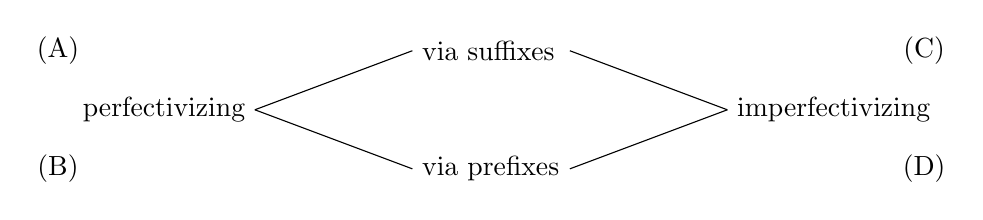
\begin{tikzpicture}
\coordinate[label=center:(A)] (A) at (-2.5,1.5);
\coordinate[label=center:(B)] (B) at (-2.5,0);
\coordinate[label=center:(C)] (C) at (8.5,1.5);
\coordinate[label=center:(D)] (D) at (8.5,0);
\coordinate[label=left:perfectivizing] (perfectivizing) at (0,.75);
\coordinate[label=right:via prefixes] (prefixesl) at (2,0);
\coordinate                           (prefixesr) at (4,0);
\coordinate[label=right:via suffixes] (suffixesl) at (2,1.5);
\coordinate                           (suffixesr) at (4,1.5);
\coordinate[label=right:imperfectivizing] (imperfectivizing) at (6,.75);

\draw (perfectivizing) -- (prefixesl);
\draw (perfectivizing) -- (suffixesl);
\draw (prefixesr) -- (imperfectivizing);
\draw (suffixesr) -- (imperfectivizing);
\end{tikzpicture} 
\end{figure}

\ili{Slavic} illustrates type (A): underived stems are predominantly \isi{imperfective} and derive a \isi{perfective} counterpart via \isi{prefixation}. Here belong the Baltic languages, Georgian, Hungarian, \ili{Yiddish}, \ili{Ossetic} and Sino-\ili{Tibetan} languages, too. By contrast, pattern (B), which includes simplexes that are predominantly \isi{imperfective}, but which derive \isi{perfective} counterparts via \isi{suffixation} – is encountered in \ili{Margi} (\ili{Chadic}) and the \ili{Micronesian} languages. More interesting is pattern (D) – simplexes are predominantly \isi{perfective} and derive \isi{imperfective} equivalents via suffixes – since it occurs in \ili{Samoyedic} languages and in Even, which are spoken in northern Eurasia. Moreover, this pattern corresponds to the prevailing strategy of Proto-Indo-European to derive “imperfectives” from “\isi{perfective}” simplexes by means of various morphological schemata most of which involve \isi{suffixation}. Pattern (C) – the same as for (D), but with prefixes – has so far remained unattested.


Second, following \citet{ArkadievShluinsky2015}, we may ask whether the language shows \isi{secondary imperfectivization} or perfectivization, i.e. whether it allows already prefixed or suffixed stems to be additionally suffixed or prefixed in order to cause a change to the opposite aspect.\footnote{We disregard the existence of double \isi{prefixation} (or ‘preverb stackingʼ) that does not change the aspect (e.g. Russ. \textit{po-ras-stavit’}{\textsuperscript{~}\PFV} ‘put each other on their places’ (distributive) ${\Leftarrow}$ \textit{ras-stavit’}{\textsuperscript{~}\PFV} ‘put on their places’). We also ignore prefixes added “on top” of already secondarily suffixed stems (e.g. Russ. \textit{po-ot-kry-va-t’}{\textsuperscript{~}\PFV} ‘open one after another’ ${\Leftarrow}$ \textit{ot-kry-va-t’}{\textsuperscript{~}\IPFV} ${\Leftarrow}$ \textit{ot-kry-t’}{\textsuperscript{~}\PFV} ‘open’). All these are cases of so-called \textit{external prefixes} among which quantifying (accumulative and distributive) functions prevail. Semantically they are of a different type, and for the system they have a different status than “simple” \isi{prefixation} and secondary \isi{suffixation}. We also neglect isolated cases and perfectivation of simplexes via suffixes. The latter is semantically restricted to semelfactives from \isi{atelic}\textsubscript{1} simplexes denoting repetitive (often cyclical, mostly motoric) action (e.g. Pol. \textit{mach-a-ć} ‘wave’ ${\Rightarrow}$ \textit{mach-ną-ć} ‘wave once’, \textit{kiw-a-ć} ‘nod’ ${\Rightarrow}$ \textit{kiw-ną-ć} ‘nod once’), though productive in these confines. See the comments in \sectref{sec:wiemerserzant:2}.} On this basis we can further distinguish whether secondary (im)perfectivization is achieved via a pair of prefixes or suffixes, or whether the secondary affix attaches to the stem from the other side of the already attached prefix or suffix, respectively. Thus, this parameter classifies according to a combination of direction of function (\isi{perfective} → \isi{imperfective} or \isi{imperfective} → \isi{perfective}) and the position of the affixes to each other (one after another or on opposite sides of the initial stem). The predominant \ili{Slavic} pattern of \isi{secondary imperfectivization} is \isi{suffixation} of already prefixed stems. Another example of this pattern is \ili{Lithuanian} (but not \ili{Latvian}; see below). \citeauthor{ArkadievShluinsky2015} do not adduce any other language with this pattern. Other languages considered by them show \isi{secondary imperfectivization} via suffixes added to other suffixes (used as perfectivizers), e.g. Kashaya and \ili{Mansi}. Chaining of suffixes is encountered for secondary perfectivization among \ili{Samoyedic} languages (like \ili{Nenets}), too. In turn, chaining of prefixes (with change of aspect) is attested in \ili{Mingrelian}.\footnote{One has to admit that the imperfectivizing prefix comes between the stem and the perfectivizing prefix (which comes first also in the “derivational history”). In the following \ili{Mingrelian} example the perfectivizing prefix is in \textbf{bold}, the imperfectivizing one is \uline{underlined}: \textit{\textbf{ge}-\uline{tmi}-a-ʒic-en-d-u}; this has to be translated as ‘was laughing at him/her’ \citep[391]{Arkadiev2014}.}

In general, however, the number of languages with any kind of secondary perfectivization or imperfectivization appears to be rather limited in contrast to the investigated sample. In particular, \citet{ArkadievShluinsky2015} argue that \ili{Latvian}, \ili{Yiddish}, Hungarian, Livonian, Georgian, \ili{Margi}, Mapuche, Aymara and the \ili{Austronesian} group do not attest such patterns. One gets the impression that many languages with a \isi{classificatory aspect system} do not have a possibility to derive another stem (belonging to the opposite aspect) from an already derived stem. However, again, the reasons (and chronology) may differ: either such a possibility was never acquired (as probably in \ili{Yiddish} or \ili{Latvian}), or it might have been lost.

If both aforementioned parameters are considered jointly, we see that \ili{Slavic} stands out against almost all areally contiguous languages and even against a larger northern Eurasian backdrop. Apart from \ili{Lithuanian}, only Istro-Romanian is known as a non-\ili{Slavic} language in which contacts with speakers of \ili{Slavic} have led to the appearance of, and increase in, secondary \isi{suffixation} (cf. \citealt{Arkadievforthcoming}
). In other words: \ili{Slavic} (plus \ili{Lithuanian} and Istro-Romanian) appear to be the only languages on a broader areal background which show productive patterns of \isi{prefixation} and (secondary) \isi{suffixation} used for the purpose of perfectivization and imperfectivization, respectively. Leaving aside now Istro-Romanian, the consistency with which this happens in \ili{Slavic} and \ili{Lithuanian} differs; \ili{Lithuanian} in many respects shows a less grammaticalized stage than the \ili{Slavic} languages which surround it. But the morphological patterns are fully parallel and some of them – such as *-\textit{āje/o-} (present)/*-\textit{ājā-} (past) and *-\textit{ēje/o-} (present)/*-\textit{ējā-} (past), discussed at length in \sectref{sec:wiemerserzant:3.2.4} – are most probably inherited from a common Baltic and \ili{Slavic} \isi{dialect continuum}. \ili{Lithuanian} has kept this “heritage” and revitalized it at a later stage with the new suffix -\textit{in\.e-}, while \ili{Latvian} has not developed any new productive aspectual \isi{suffixation} which would go beyond strong lexical restrictions (see \sectref{sec:wiemerserzant:5.4}).\footnote{It did, however, create a somewhat productive suffix \textit{-inā-} to derive morphological causatives and other deverbatives.} For example, the common suffix (*-\textit{āje/o-}...) is retained in just a few verbs such as \textit{brauk-t} ‘drive-\textsc{inf}’ vs. \textit{brauk-ā-t} ‘drive-\textsc{hab-inf}’.

To conclude, crucial for the rise of the \ili{Slavic} \isi{aspect system} based on \isi{stem derivation} was the fact that one productive set of affixes (\isi{prefixation}) at some point in history started being combined with another productive set of affixes (suffixes). It follows from the areal overview given above that these morphological preconditions are met only rarely in languages of the world. It is our conviction that this constellation is the key to understanding the rise of the \ili{Slavic} \isi{aspect system}. Above we have traced back the development of \isi{prefixation} and \isi{suffixation} of verb stems and argued that they developed from separate sources and diachronically at different periods of time: imperfectivization schemata represent old – albeit highly remodelled – patterns while the exploitation of prefixes for perfectivization is a much more recent development. In contrast, other IE languages in Europe that have exploited \isi{prefixation} to code actionality (which is a pre-stage to aspect) have lost the old imperfectivization strategies altogether. This topic will be addressed in the next section.

\section{Verb stem derivation in ancient Indo-European languages of Europe}\label{sec:wiemerserzant:5}

In \sectref{sec:wiemerserzant:3}, we supplied a diachronic account of verbal \isi{prefixation} and \isi{suffixation} in \ili{Slavic}. In turn, the preceding discussion in \sectref{sec:wiemerserzant:4} served the purpose of recognizing the typological peculiarities of \ili{Slavic} aspect and of relativizing claims concerning its alleged rarity. In this section, we want to critically assess some facts and findings that help cast light on the role verbal affixation might have played in shaping the \isi{aspectual character} of verb stems in other IE languages outside of \ili{Slavic}. Our survey is selective: we do not pretend to give an exhaustive account of \isi{preverbation} and \isi{prefixation} (or of \isi{suffixation}) in these languages, but we focus on languages (or language groups) with some closer areal affinity to at least some \ili{Slavic}-speaking territory during the first millenium AD.

Many scholars have mentioned the widespread existence of \isi{preverbs} (often also included into inventories of particles) attached to verbal stems in different old IE languages of Europe. The morphological status of these \isi{preverbs} varies, as they are sometimes characterized as proclitics, on other occasions as already tightly agglutinated parts of verbal stems, i.e. as prefixes. Possibly, this variation reflects different stages on a clitic-affix cline of morphologization. Admittedly, there is no straightforward correlation between this assumed cline and the development of a preverb into a prefix. One of the problems is that neither \isi{preverbs} nor prefixes need be unstressed, so that we cannot be sure that it is cliticization as such which triggers the processes.\footnote{We want to thank Christian Lehmann for pointing this out to us.} In the first place, however, tightness of \isi{coalescence} with lexical stems does not \textit{per se} give reliable information concerning the function of morphemes on a preverb~{\textgreater}~prefix-cline and their role in forming systematic oppositions pertaining to actionality and/or grammatical aspect. Note that investigations into \isi{preverbation} in ancient IE languages have concentrated largely on issues of morphologization (cliticization {\textgreater} agglutination) of \isi{preverbs} originating from adverbs or so-called \textit{verb particles} and on the question of what processes of \isi{coalescence} tell us about constituent and argument structure in early IE.\footnote{Cf. for instance, \citet{Vincent1999} on \ili{Latin} and \ili{Romance}, \citet{Boley2004,Cuzzolin2006} more generally on \isi{preverbation} in diverse stages of early IE languages. Among others, \citet{Luraghi2003} and \citet{Viti2008} investigated the role of spatial prefixes, their relation to cognate prepositions and adverbs as well as their role in the syntax of Ancient Greek. As for \ili{Latin} cf. \citet[557--566]{Leumann1977[1926]}
 and \citet{Haverling2003}.}  Preverbs as mere aspectual bounders are mentioned rather occasionally, so that it is hardly possible to draw any conclusions as to whether the bounder function should be characterized as modification or as telicization\textsubscript{2}; cf. for instance, \citet[10]{Cuzzolin2006}. Among others, this applies to Ancient Greek, too, and for this reason we will not deal specifically with Greek anymore in this article.

\subsection{Romance}\label{sec:wiemerserzant:5.1}

This general picture obviously holds true also for \ili{Latin}. In Classical \ili{Latin}, many prefixes still functioned as markers of \isi{telicity}\textsubscript{1}, but this function deteriorated by Late \ili{Latin} (after 300 AD; cf. \citealt{Haverling2003}), thus more or less at the time of the Great Migrations. Therefore, we feel justified to say that, by and large, neither \ili{Romance} nor its ancestor \ili{Latin} pushed the use of \isi{preverbs} further than the modificational stage (see the upper part of \tabref{tab:wiemerserzant:4}) and maybe some incipient stage (ii).

In the \ili{Romance} successor languages of \ili{Latin}, prefixes usually became lexicalized and opaque when they could no longer be separated from the stem; compare It. \textit{in{\textbar}segnare} ‘teach’, Fr. \textit{s’en{\textbar}dormir} ‘fall asleep’ (\citealt[125]{Haverling2003}; \citealt[12]{Cuzzolin2006}), or the prefixes used did not carry any aspectual function, being restricted, as a rule, to spatial and related functions (e.g. It. \textit{ag-giungere—dis-giungere} ‘add, attach—separate’) or to \isi{comitative} meaning or redoing (compare \ili{Romance} \textit{re}-, \textit{con}- and their translational equivalents). Obviously, in older stages of \ili{Romance}, e.g. Old French, \isi{preverbs} were used widely, but according to the examples adduced in relevant publications (e.g., \citealt{Dufresne2003}) the function of these \isi{preverbs} was restricted to modifications of the verbal action more or less like in modern \ili{German} or Dutch.


Suffixes, in turn, proved unproductive, or they were incorporated into \isi{inflectional} paradigms. The latter happened to \ili{Latin} -\textit{sc}-, which occurs in some forms of the present \isi{tense} conjugations of \ili{Romance} successor languages (e.g., It. \textit{capi-sc-e} ‘s/he understands’ from \textit{cap-ire}.\textsc{inf} ‘understand’). Cf. \citet{Allen1995} on this process whereby a former derivational morpheme turns into a merely formal marker incorporated into \isi{inflectional} paradigms. In \citet{Greenberg1991} this process was called \textit{regrammaticalization}. As we saw in the preceding sections, this is clearly not what happens when we distinguish \isi{perfective} and \isi{imperfective} stems. Only the development of the \ili{Slavic} imperfect shows a change from \isi{derivation} into inflection (see \sectref{sec:wiemerserzant:3.2.4}).

In sum, neither (late) \ili{Latin} nor its \ili{Romance} successor languages relied on productive \isi{prefixation} strategies to code \isi{telicity}\textsubscript{1}. The same applies, \textit{mutatis mutandis}, to \isi{suffixation} strategies to mark actionality functions associated to imperfectivity. We are unaware of any reliable findings concerning possible contact relations of Vulgar \ili{Latin} or its successor varieties in early \ili{Romance} with \ili{Slavic}. We thus refrain here from any comments on this issue.

\subsection{Celtic}\label{sec:wiemerserzant:5.2}

It is not entirely clear whether there were considerable contacts between \ili{Celtic} and \ili{Slavic} populations, in particular during the Great Migrations (cf. the critical remarks in \citealt[64--69]{Polomé1972} and \citealt[48]{Andersen2003}). Although toponyms of \ili{Celtic} origin have been attested as far east as in the \ili{Danubian} delta and the upper Dniester basin \citep{Blažek2015}, these traits of \ili{Celtic} influence could have been due to settlements from the last centuries BC, when \ili{Celtic} tribes had spread over vast territories of Europe and into Asia Minor. In fact, “\ili{Celtic} speech, apart from possible enclaves, appears to have died out on the European continent by AD 500” (\citealt[2]{MacAulay1992}), and the earliest form of \ili{Celtic} that could be reconstructed more or less completely from extant sources, Old \ili{Irish}, reflects a stage just after this time (approx. 6th-9th century AD; \citealt[1--11]{Thurneysen1975[1946]}). Moreover, Old \ili{Irish} was spoken in the northwestern periphery of an earlier \ili{Celtic} \isi{dialect continuum}, while contacts with Slavs could have occurred only on its opposite end, and we do not know to which extent other \ili{Celtic} dialects were comparable to Old \ili{Irish} in terms of \isi{preverbation} (or \isi{suffixation}). \citet{Gvozdanović2009,Gvozdanović2015} wonders whether certain important typological changes in word prosody such as syllable structure and the direction of palatalization from regressive to progressive assimilation of the velars /\textit{k}/, /\textit{g}/, /\textit{x}/ could not have been due to some \ili{Celtic} influence. She links her argument to the Venetian region to which \ili{Celtic} is supposed to have once spread. However, apart from Gvozdanović’s observations on phonology (mainly word prosody) there are no really “hard core” arguments able to substantiate \ili{Celtic} influence on \ili{Slavic}. After all, “we do not have sufficient evidence to identify the individual contacting language, which may well have been the eastern European Venetic […] of which we have no direct linguistic evidence” \citep[97]{Gvozdanović2015}. The relation to \ili{Celtic}, thus, remains unclear.

Therefore, the following brief remarks on \isi{preverbation} in Old \ili{Irish} have to be taken with caution, at least insofar as we cannot say whether Old \ili{Irish} did not differ, with respect to verbal \isi{stem derivation}, from \ili{Celtic} varieties which previously had been spoken on the European continent, some of them possibly in some proximity to speakers of Common \ili{Slavic}.

Old \ili{Irish} had some dozen \isi{preverbs} (prefixes), most of them obviously in a transitional stage between clitics and affixes; the most widespread and prominent was \textit{ro}-. \citet[104]{Gvozdanović2015}, summarizing \citet[339--348]{Thurneysen1975[1946]}, concludes that Old \ili{Irish} \textit{ro-} “perfectivizes the verb on the level of grammatical aspect, not only \isi{lexical aspect}”. She even goes further saying that the functional properties of this preverb, “as part of the verb phrase, are fully paralleled by the perfective aspect\is{perfective} in \ili{Slavic}”. These parallels concern the combination with the imperfect, which yields repetition in the past (compare modern \ili{Bulgarian}, see \sectref{sec:wiemerserzant:3.2.5}), and, first of all, \isi{prefixation} of present \isi{tense} stems which occurred only in gnomic or other inactual functions of the present (including dispositional modality, e.g. \textit{asˑ\textbf{{ro}}-b(a)ir} ‘can [= is able to] sayʼ vs. \textit{asˑbeir} ‘saysʼ). However, the term \textit{perfective} probably entered the English translation of Thurneysen’s authoritative grammar (written originally in \ili{German}) as an inadequate rendition of Germ. \textit{perfektisch} or \textit{Perfekt} (\citealt[251]{Lambert1995}, following \citealt{McCone1987}),\footnote{Cf. \citet[319]{Thurneysen1909}. According to \citet[252]{West1981-1982}, the facts allow for an interpretation as mere anteriority marker as well, so that stems prefixed with \textit{ro}- should probably be considered ‘perfect forms’.} where it seems to mean accomplished action (Germ. \textit{vollendete Handlung}), i.e. \isi{telic}\textsubscript{2} \isi{predicates}. Moreover, \textit{ro}- (leaving aside other \isi{preverbs}) was optional, verbs with an inherently \isi{telic} meaning (= \isi{telic}\textsubscript{1}) could convey \isi{perfective} values without \textit{ro}- as well (cf. \citealt[141f., 245--248]{Lewis1937}; \citealt[231--239]{Lambert1995}). For this reason, \citet[81]{Schumacher2004} proposed to consider \textit{ro}- (and other \isi{preverbs}) just as an augment of the stem that does not constitute any new category (differently \citealt[251f.]{Lambert1995}).

These observations, as fragmentary as they are, seem to be indicative rather of a stage in which \isi{preverbs} (prefixes) frequently but optionally were used to mark inherent boundaries, i.e. to create \isi{telic}\textsubscript{2}-\isi{predicates} under favorable conditions and independently from \isi{tense}. This corresponds to stage (ii) in \tabref{tab:wiemerserzant:4}. This resembles the situation we encounter in \ili{Gothic}, to which we now turn.

\subsection{Gothic}\label{sec:wiemerserzant:5.3}

\ili{Germanic} has been regarded as being much closer to \ili{Slavic} and Baltic than any other of the IE groups in Europe. It is very probable that the speakers of \ili{Gothic}, as the best-documented old \ili{Germanic} language, were in rather close contact with Baltic and \ili{Slavic} tribes, before they fell victim to the Great Migration (in which they intensely participated), so that by the 6th c. AD they disappeared from history in eastern Europe \citep[13–15]{Kotin2012}, while the Visigoths on the Iberian Peninsula eventually abandoned their language at the beginning of the 7th c. AD.

The \ili{Gothic} verbal prefix \textit{ga}- was the most salient representative of a series of prefixes, and its behavior was very similar to Old \ili{Irish} \textit{ro}-.\footnote{The same applies to Old High \ili{German} (\textit{gi}-) and other prefixes in the most ancient stages of documented \ili{Germanic} languages (on which cf. \citealt[297, 397]{Kotin2012}).} The known documents (primarily Wulfila’s Bible) reflect the state of the language from approx. the 4th c. AD (i.e. slightly earlier than Old \ili{Irish}). These doculects were, of course, influenced especially by Greek, and also by \ili{Latin} \citep[21]{Kotin2012}. In particular verb stems prefixed with \textit{ga}- have, since \citet{Streitberg1891}, been evoking divergent claims about their status as “perfectivizers”. As with the Old \ili{Irish} \isi{preverbs}, most researchers (except \citealt{Maslov1959}) have remained rather vague as for what they understand by \textit{aspect}, in particular which role is played by prefixes, and whether the designation \textit{perfective} characterizes a lexical or a grammatical feature. In \ili{Gothic}, \textit{ga}- and some more prefixes\footnote{\citet[393f.]{Kotin2012} names \textit{dis}-, \textit{fra}-, \textit{faír}-, \textit{ga}-, his examples also show \textit{us}- (\citeyear[397]{Kotin2012}), cf. also \citet[205--209]{Guxman1998}. \citet[124]{Braune1961} name some more, and they mention tmesis and other signs of a looser juncture between prefix and stem (ibid: 124–125).} functioned not only as lexical modifiers, but they often fulfilled functions that are reminiscent of mere bounders of the action denoted by the \isi{simplex stem} (see below). Thus, \citet[287]{Kotin2012} writes that \ili{Gothic} demonstrated “a relatively stable opposition of simplexes and so-called \textit{ga}-composites […], that can largely be interpreted as aspectual” (our translation). However, \textit{aspectual} here does not have the value of a grammatical opposition, but, rather, of a complex of actional and voice-related features. Remarkably, \citeauthor{Kotin2012} also mentions that in quite a few cases, prefixes did not so much modify the lexical semantics of the simplex, but rather made it more pronounced; conversely, some simplex stems “selected” a prefix depending on their own inherent semantics (\citeyear[394–395]{Kotin2012}).\footnote{With the exception of \textit{ga}-, \citet[394]{Kotin2012} ascribed a prototypical semantic function to each particular prefix: „in connection with various verb stems this function could either have remained practically unaltered, or it was modified to different degrees, depending on the modifications allowed or even required by the semantics of the verb stem. This property of the derivational basis exerts an impact not only on modifications of the basic semantic function of the prefix, but it also restricts the selection of the latter.” (our translation) For instance, \textit{taíran} ‘tearʼ ${\Rightarrow}$ \textit{dis-taíran} (${\approx}$ \textit{ga-taíran}) ‘dittoʼ, \textit{qistjan} ‘destroyʼ ${\Rightarrow}$ \textit{fra-qistjan} ‘dittoʼ: \textit{dis}- was lexically associated with separation, \textit{fra}- with destruction and loss (\citeyear[394–395]{Kotin2012}).} This observation brings to mind the Vey-Schooneveld effect of prefixes discussed in \sectref{sec:wiemerserzant:3.2.2}.

However, even if we regard \textit{ga}- as a perfectivizer proper, its application remained restricted both in terms of the range of verb stems with which it could be combined (type-frequency) and the reliability with which it was encountered in cases when it should be expected from the meaning in discourse (token-fre\-quen\-cy). The application of \textit{ga}- (or any other prefix) was by no means very consistent. Moreover, the extant texts do not allow for too far-reaching conclusions about which pairs of simplex/prefixed stems were distributed over different aspectual functions, in particular as concerns finite forms (cf. also \citealt[250f.]{West1981-1982} and the review of the literature until the mid-1950s in \citealt{Maslov1959}). It is symptomatic that even Kotin’s thorough examination of \ili{Gothic} texts brought to light such pairs only for inherently \isi{telic}\textsubscript{1} verbs (cf. \textit{ga-swiltan} vs. \textit{swiltan} ‘die – be dying [Germ. \textit{im Sterben liegen}]ʼ, \textit{fullnan} ‘fill [\textsc{intr]}ʼ vs. \textit{ga-fullnan} ‘fill [\textsc{intr]}, become full (to its limits)ʼ) and for verbs of passive perception (e.g. \textit{saíƕan} ‘seeʼ vs. \textit{ga-saíƕan} ‘catch sight of [Germ. \textit{erblicken}]ʼ). With these verbs, \textit{ga}- served to mark off the initial boundary of the perceptual state (= \isi{atelic}\textsubscript{1}), whereas with \isi{telic}\textsubscript{1} verbs, namely those denoting more punctual changes \textit{ga}- modified the lexical meaning (e.g. \textit{niman} ‘takeʼ vs. \textit{ga-niman} ‘take with o.s., take alongʼ, \textit{qiman} ‘come, arriveʼ vs. \textit{ga-qiman} ‘gather, assemble [\textsc{intr]}ʼ); cf. \citet[294--300, 395--397]{Kotin2012}. 

In sum: it is not entirely clear whether \ili{Gothic} \textit{ga-} should be analyzed as a marker of \isi{telicity}\textsubscript{1} or \isi{telicity}\textsubscript{2}, not least due to some terminological confusion in the literature. Examples such as Kotin’s \textit{bindan} ${\Rightarrow}$ \textit{ga-bindan} ‘bind, tie (up)ʼ, \textit{swiltan} ${\Rightarrow}$ \textit{ga-wiltan} ‘dieʼ (see above) suggest that there was, at least, a considerable progress from \isi{telicity}\textsubscript{1} towards \isi{telicity}\textsubscript{2} in \ili{Gothic} (our stage (ii) in \tabref{tab:wiemerserzant:4} above).{} By contrast, \citegen{Maslov1959} analysis leads rather to\largerpage a characterisation of \textit{ga}- as a marker of \isi{telicity}\textsubscript{1} (stage (i) in \tabref{tab:wiemerserzant:4}).

\subsection{Baltic}\label{sec:wiemerserzant:5.4}

The morphological prerequisites necessary for the innovations common to all later \ili{Slavic} languages are present in Baltic as well. This allows to infer that the premises of these innovations must have developed in a larger dialectal region of early IE, of which \ili{Slavic} and Baltic formed part. Concomitantly, the old layer of Baltic \isi{suffixation} is etymologically related to the respective old layer of \ili{Slavic} (see \sectref{sec:wiemerserzant:3.2.1} and \sectref{sec:wiemerserzant:3.2.4}). However, old suffixes have ceased to be productive. While varieties of \ili{Lithuanian} created new productive suffixes such as \textit{-in\.e-} (iterative, durative, etc.) or \textit{-dav-} (habitual past), \ili{Latvian} did not introduce new verbal suffixes with aspectual functions.

\ili{Latvian} shows a certain opposition of \isi{atelic}\textsubscript{2}/\isi{telic}\textsubscript{2} \isi{predicates} comprising non-punctual \isi{telic}\textsubscript{1}-verbs. This opposition is lexically restricted and builds on prefixed stems contrasted with the respective simplex stems that take verb particles part of which are cognates of the prefixes; for instance,
\textit{\textbf{ie}-nāca istabā} 
‘in-come.\textsc{pst.3} room.\textsc{loc.sg}’ 
‘entered into the room’ (usually \isi{telic}\textsubscript{2}) 
vs. 
\textit{nāca \textbf{iekšā} istabā} 
‘come.\textsc{pst.3} inside.\textsc{prt} room.\textsc{loc.sg}’ 
‘was entering the room’ (\isi{telic}\textsubscript{1}); cf. \citet[132–141]{Holvoet2001}, \citet[132–134]{Arkadiev2015}. Verb particles are a relatively recent phenomenon, which most probably arose from contact with \ili{Germanic} (Low and High \ili{German}, \ili{Swedish}) and \ili{Finnic} \citep{Wälchli2001}.\footnote{There is much of mutual influence between \ili{Latvian} and \ili{Finnic} (Estonian, Livonian) contact in here, and Estonian, in turn, is probable to have introduced this technique under contact with \ili{Germanic} (\citealt{Hasselblatt1990}; \citealt{Metslang2001}). Anyway, this recent innovation is in stark contrast to the otherwise strong suffixing strategy of Finno-Ugric.}

\ili{Lithuanian} is different, since in its Aukštaitian dialects and the standard language it has introduced two new suffixes relevant for differentiation in actionality: semelfactive -\textit{\.ere-/-\.ele}- and -\textit{(d)in\.e}-; the latter takes on functions associated to unboundedness.\footnote{Both suffixes certainly arose from some morphological reanalysis (as did most of the \ili{Slavic} suffixes mentioned in \sectref{sec:wiemerserzant:3.2.3}).} Remarkably, especially the latter suffix has been attested as particularly frequent (on type and token level) in southeastern Lithuania, i.e. in close vicinity with (East) \ili{Slavic}. The suffix -\textit{(d)in\.e-} has been extraordinarily frequent in (now extinct or moribund) insular dialects in Belarus. It is thus apparent that this new suffix gained frequency from contact with \ili{Slavic} speakers (and \ili{Lithuanian}-East \ili{Slavic} bilingualism), but only in recent times (\citealt[359--363]{Wiemer2009}; \citealt[125--131]{Arkadiev2015}). The same may hold true for double \isi{prefixation}, which is otherwise unusual in \ili{Lithuanian} and Baltic in general, but quite widespread in East \ili{Slavic}. It would be risky to try to extrapolate into a remote past these facts about the distribution\largerpage and frequency of these younger verbal affixes that are relevant for aspectual \isi{distinctions}. 

\section{Conclusion and an outlook}\label{sec:wiemerserzant:6}

In this paper it has been our main concern to give a comprehensive assessment of the internal preconditions which made the rise of the contemporary \isi{aspect system} based on \isi{stem derivation} (\isi{perfective}/\isi{imperfective} verbs) of \ili{Slavic} languages possible. We have restricted ourselves to the core of the system and inquired into morphological changes that affected the formation of verb stems in the prehistory and early history of \ili{Slavic}. The analysis concerned both particular morphemes and patterns of affixation in relation to each other and to initial verb stems; we tried to trace back these patterns and morphemes from PIE into \ili{Slavic}, pointed out genuinely \ili{Slavic} innovations based on an IE heritage and discussed the further expansion or loss of early inner-\ili{Slavic} developments. We have focused on changes that affected \ili{Slavic} as a whole and stopped short at the point when, after the consolidation of the core system, inner-\ili{Slavic} differences both in formal expression and in the range and hierarchy of functions became more pronounced.

Favorable inherited conditions are visible in the internal changes of \ili{Slavic} since times prior to documentation (see \sectref{sec:wiemerserzant:3}). In asking whether or not \ili{Slavic} aspect continues aspectually relevant oppositions found in PIE (cf. \textit{inter alia}, \citealt{vanWijk1929}; \citealt{Stang1942}) we have to be careful not to mix up morphological schemata with functions of grammatical aspect or aspectual functions in general. Once this is taken into account, we can claim that the morphological devices used in Common \ili{Slavic} to mark unboundedness \textit{grosso modo} represent – albeit highly restructured and modified – heritage from late PIE. An important feature of \ili{Slavic} morphemes to mark unboundedness is that there is a strong tendency towards morphological concatenation, away from non-concatenative PIE schemata. This trend can be reconstructed for Common \ili{Slavic} and it continues to this day.

Preverbation (particles, prefixes and intermediate stages) developed at the time of ancient IE languages. Especially the comparison with Old \ili{Irish} (see \sectref{sec:wiemerserzant:5.2}) demonstrates that \isi{preverbs} used as bounders of verbal action evolved in very different regions of Europe by the middle of the first millenium AD. Whether this testifies to spontaneous independent parallelism triggered by some propensity on the basis of inherited adverbs or should rather be explained by mutual contacts between subgroups in Europe (e.g. between early \ili{Slavic} and \ili{Gothic}), cannot be ascertained. However, \isi{preverbation} has been prominent especially for changes of valency or argument structure whereas, apparently, apart from \ili{Slavic}, in none of these IE languages did prefixes (or other \isi{preverbs}) start to productively function as mere bounders of verbal action, without additional functions on the syntax-semantics interface. These patterns were then, in \ili{Slavic}, strengthened by the combination with suffixes, which decayed in other IE languages of Europe.

Thus, for late Common \ili{Slavic} we can also assume a tendency of extending the distinction between \isi{telic} and \isi{atelic} stems from a purely lexical opposition (i.e. from \isi{telic}\textsubscript{1} vs. \isi{atelic}\textsubscript{1}) into an opposition in which realized \isi{telicity} (= \isi{telic}\textsubscript{2} meanings) is marked via \isi{prefixation}. At a later stage, prefixes start serving also the differentiation of other aspectual meanings such as ingressivity or mere temporal delimitation (see \tabref{tab:wiemerserzant:4} in \sectref{sec:wiemerserzant:3.2.2}). Simplexes, unmarked also with respect to \isi{telicity}\textsubscript{2} (as there were both \isi{telic}\textsubscript{1} or \isi{atelic}\textsubscript{1} simplexes to begin with), underwent different, lexeme-specific developments still into recent centuries to stabilize aspect assignment of stems. Unprefixed, but suffixed stems – representing the oldest layer – played a subsidiary role in the emergence of the opposition. From the point of view of morphological patterns, the last step was taken when suffixes started being productively attached to already prefixed stems (so-called \textit{secondary imperfectivization}). This pattern has remained less productive in the western half of \ili{Slavic}, while it is very prominent in the eastern half (East \ili{Slavic}, \ili{Bulgarian}, \ili{Polish}).

This being settled, a further aim of this paper consisted in demonstrating that, although \ili{Slavic} is by no means unique in having developed a \isi{classificatory aspect system}, it nevertheless stands out on a larger areal, namely Eurasian, background and in comparison to other IE groups in Europe. We thus compared diachronic and synchronic data of \ili{Slavic} with somewhat fragmentary data against an areal and typological backdrop (\sectref{sec:wiemerserzant:4}) as well as with likewise fragmentary data from earlier stages of IE languages (\sectref{sec:wiemerserzant:5}).

Now, on the basis of this comparison, there arises a more intricate question, which, for the moment, we only want to state. Namely: one wonders to what extent the rise and consolidation of the \ili{Slavic} \isi{aspect system} can be explained as only a spontaneous evolution that just continued already existing preconditions of \isi{stem derivation}. To what extent might contact with non-IE-speaking populations have helped trigger, or support, the consolidation of such continued development, which we do not find in areally close IE languages? To put it differently: there is no doubt that the morphological prerequisites necessary for the evolution of stem-derivational aspect in \ili{Slavic} continued earlier patterns that were partly rooted in PIE. But why has only \ili{Slavic} developed these prerequisites in such a consistent manner during the last, say, two millenia, whereas in other IE groups \isi{suffixation} and/or \isi{preverbation} have gone other ways? In the latter, such prerequisites disappeared or were renewed (for instance, by separable verb particles), but nowhere else have prefixes and suffixes come together to jointly build a grammatical system as in the \ili{Slavic} languages (except for much more recent developments as in some varieties of \ili{Lithuanian}, obviously under East \ili{Slavic} influence; see \sectref{sec:wiemerserzant:5.4}).

\ili{Slavic} expanded over a large territory all over eastern Europe since about 600 AD; contacts with groups of speakers of \ili{Uralic} or \ili{Turkic} were, thus, very likely. In general, the existence of Finno-Ugric and \ili{Turkic} adstrata and even substrata in the eastern part of \ili{Slavic} can hardly be doubted.\footnote{Cf. \citet{Veenker1967} and \citet{Haarmann2014} on Finno-Ugric, \citet{Stachowski2014} on \ili{Turkic}. Consider also the history of the Bulgars from the middle of the first millenium AD, a \ili{Turkic} (Oghur) tribal union which was later ethnically and linguistically assimilated by eastern South \ili{Slavic} people and henceforth gave its name to this mixed population and the later state.} However, whether contact with Finno-Ugric or \ili{Turkic}-speaking populations might have been sufficient to strengthen suffixing strategies must be inquired in a well-considered manner, taking into account various kinds of (often indirect) evidence and equilibrating findings from different approaches. Among other things, it should be asked what morphological techniques of stem extension in possible contact languages looked like, which types were productive and resembled, in some way or other, \isi{stem derivation} in early \ili{Slavic}. For instance, according to Serebrennikov, many Finno-Ugric languages show suffixal extensions of verb stems with various functions from the domains of iterativity (repetitive or habitual action) or of semelfactivity. These aspectual meanings can be interpreted as remnants of an earlier stage, when dialectal differentiation was less advanced (\citealt[31–34, 188]{Serebrennikov1960}). 

As concerns \ili{Turkic}, we may assume that its oldest reconstructable layer “operated entirely by adding suffixes at the end of the word and had a fully developed system of suffixes” \citep[27]{Clauson1962}. Throughout, \ili{Turkic} languages have experienced several renewals of \isi{suffixation}, among others of suffixes modifying the \isi{aspectual character} of the verb. Such suffixes developed via morphologization (enclisis {\textgreater} agglutination) from converb or \isi{auxiliary} constructions (\citealt[41--43]{Johanson1998a}, \citeyear*{Johanson1998b}: 113--115; cf. also \citealt[262--272]{Erdal2004}). In general, \ili{Turkic} languages can be regarded as having remained astonishingly homogeneous in this respect (\citealt[181]{Menges1968}; \citealt[111]{Johanson1998b}). One wonders whether such findings cannot be more substantiated with respect to aspectual functions of suffixes (or postverbs, which preceded them in morphologization) at the dawn of written documentation of \ili{Turkic}, i.e. from the early eight century AD, and in subsequent centuries. One should seek contacts of \ili{Uralic} and \ili{Turkic} speaking populations especially for the Common \ili{Slavic} period (400–900 AD), when the \ili{Slavic} \isi{dialect continuum} must have been still sufficiently homogeneous and compact for innovations to spread across \ili{Slavic} from East to West, including the strengthening of already developed patterns.

Now, if we want to explain the early stages in the rise of the \ili{Slavic} \isi{perfective}/\isi{imperfective} opposition, we should take into account the following considerations: (i) In contrast to many other IE languages, \ili{Slavic} has partly preserved stem extensional patterns (suffixing strategies, though less concatenative), (ii) frequent patterns of \isi{preverbation} (\isi{prefixation}) in later IE languages in Europe outside \ili{Slavic} did not further participate in the formation of viewpoint aspect despite some incipient developments, and (iii) the predominant suffixing strategies of non-IE languages with which speakers of prehistoric and later \ili{Slavic} must have come into considerable contact, in particular since the Great Migrations. Considering all these pieces of a puzzle, one is tempted to formulate the following hypothesis:
\ea
 While, during the first millenium AD, \isi{prefixation} of verb stems was shared with other IE language groups as a new development in Europe, \isi{suffixation} patterns were sustained by similar patterns in Finno-Ugric and \ili{Turkic} speaking populations.
\z
\noindent 
 In some sense, Common \ili{Slavic} came to be sandwiched between an area with predominant preverbalizing strategies in the IE speaking West and an area with a clear preference for suffixing strategies in the East where speakers of Finno-Ugric and \ili{Turkic} dominated. The morphological prerequisites for a system of viewpoint aspect based on the combination of prefixes and suffixes in verbal \isi{stem derivation} had developed by Common \ili{Slavic} times, but \textit{only} in \ili{Slavic} \textit{both} suffixes and prefixes eventually turned out as being capable of marking aspectual \isi{distinctions} without voice or valency-related changes. Support for this assumption comes from the observation that secondary \isi{suffixation} has been much more productive in the eastern half of \ili{Slavic} than in the western one (see \sectref{sec:wiemerserzant:3.2.3}).

This hypothesis and the issues related to it wait for an investigation, if one wishes to complement an internal reconstruction with contact-induced considerations. 

\section*{Acknowledgments}
First and foremost, we are obliged to Bridget Drinka, who not only helped smooth the style of the exposition, but contributed a lot of valuable remarks concerning Indo-European and other issues. We also owe special gratitude to Peter Arkadiev and Christian Lehmann, whose comments on an earlier version of this article made us aware not only of some unfortunate formulations but, first of all, of pitfalls and fallacies which we had overlooked. Furthermore, we have to thank (alphabetically) Henning Andersen, Walter Breu, Pino Marco Pizzo and Florian Sommer, who drew our attention to other possible pitfalls. Beyond them, we want to thank Silvia Luraghi and Chiara Zanchi for discussion of Ancient Greek (which remained in the background), Östen Dahl and Ljuba Veselinova for discussion of typological matters, Bohumil Vykypěl for some advice concerning sources of prehistoric \ili{Slavic} morphology, Jadranka Gvozdanović and Ranko Matasović concerning \ili{Celtic} and Lázsló Károly concerning \ili{Turkic}. Needless to say, none of these colleagues should be made responsible for any possible drawbacks of this article, as the sole responsibility for any remaining misinterpretations or mistakes is ours.

\section*{Abbreviations} 
\begin{tabularx}{.45\textwidth}{@{}>{\scshape}lX}
acc & accusative\\
act &  active\\
dat  & {dative}\\
f  & feminine\\
hab &  habitual\\
impf &  imperfect\\
indef  & indefinite\\
inf  & {infinitive}\\
intr  &      {intransitive}\\
n &  neuter\\
neg & negation\\
nom  & {nominative}\\
nprs  &        non-present stem\\
\end{tabularx}
\begin{tabularx}{.5\textwidth}{>{\scshape}ll@{}}
pfx   &       prefix\\
pl &  plural\\
prs &  present\\
pst &  past\\
q  & question particle\\
redupl &  reduplication\\
rfl &  reflexive\\
sfx  &        suffix\\
sg &  singular\\
thv   &       {thematic vowel}\\
unbound.pst  &  marked unbounded past\\
vir &  virile\\
voc  & vocative\\
\end{tabularx}

{\sloppy
\printbibliography[heading=subbibliography,notkeyword=this]
}
\end{document}